\chapter{Multigroup Reactor Methodology}
\index{Multigroup Reactor Methodology@\emph{Multigroup Reactor Methodology}}

\section{Introduction}
\index{Introduction@\emph{Introduction}}
Previous studies have examined the use quickly executing, dominant physics codes for use in the
nuclear fuel cycle.  Unlike analytic techniques (such as neutron transport) which seek to completely 
solve fundemental physical systems, dominant physics codes parameterize the system and use interpolations
of results from stricter analytic methods to form a quick, run-time solution to the system at hand.

Dominant physics methods may be used for any fuel cycle component: enrichment, reactors, reprocesing, 
repositories, \emph{etc}.  However, their greatest advantage comes for such components whose analytic
techniques are computationally intensive.  Thus previous work has focused on reactors and repositories.

The dominant physics reactor methodologies to date have been one-energy group, fluenece-based parameterizations.
Neutron production \& destruction rates and transmutation matrices as a function of fluence 
(time-integrated flux) were recorded for each species initial present in the core.  A linear combination of 
the inital nuclides was then used to compute the multiplication factor, fuel burnup, and used fuel 
vector at discharge.

Unfortunately, because of the constant flux irradiation method used to generate the parameterizations, 
the above model was not sensitive to changes in the flux spectrum over the course of the burn.  The 
requirement of a static flux spectrum limits the type of reactors that may be studied using such a 
dominant physics methodology.  In seeking to expand the types of reactors model-able from the 
current fast reactors and light-water reactors, the flux spectrum must be folded back into the 
underlying parameterization.


\section{Multigroup Cross Section Generation}
\index{Multigroup Cross Section Generatrion@\emph{Multigroup Cross Section Generation}}
When seeking to parameterize nuclear power reactors as a function of initial conditions, 
the set of possible independent parameters quickly becomes large. In addition to geometric 
design considerations, the fuel characteristics of the reactor must also be accounted for.

In the one-energy-group reactor model (R1G), the initial loading was parameterized based
on neutron production rates, neutron destruction rates, and transmutation matrices per
nuclide \cite{Scopatz2009d}.  All of these metrics are a function of flunece.  (Under 
constant irradiation, fluence is a clear surrogate for time.)

A $G$-energy-group reactor model (RMG) seeks to re-parameterize the one-group formulation 
in terms of energy.  While the multi-group formulation will remain on a per nuclide basis, 
the neutron reaction rates do not have have a meaningful per unit energy expression that 
is independent of the flux.  Moreover changing reaction rates also invalidate the 
transmutation matrices.  

Therefore, the RMG, in a level of sophistication above the R1G, must be able to calculate
the multigroup flux spectrum.  To do so requires multigroup microscopic neutron cross-sections.  
Using the cross-sections as independent reactor parameters in a multigroup sense is 
effectively equivalent to removing the flux from the reaction rates in the one-group case.
This is seen in Equation \ref{reaction_rate_calc}
\begin{equation}
\label{reaction_rate_calc}
R = \sigma \cdot \phi \cdot 10^{-24}
\end{equation}
where $R$ [hz] is the reaction rate, $\sigma$ [barns] is the one-group cross section, and
$\phi$ [n/cm\superscript{2}/s] is the energy-integrated flux.

The remainder of this section is delineated into a discussion on notation, how initial 
reactor conditions are specified, the three methods that were used to compute the
cross sections, and the validation technique used.

\subsection{Notation}
\index{Notation@\emph{Notation}}
The group constants $\sigma_{itg}$ or $\sigma_{ipg}$ are themselves parameterized by nuclide, 
time or perturbation (see following section), and  incident neutron energy.  Nuclides are indexed by 
$i$, times are indexed by $t$, perturbations are indexed by $p$, and energy is indexed by $g$ with 
lower indices representing higher energy groups.

\begin{table}[htbp]
\begin{center}
\caption{Neutron Reaction Types}
\label{reaction_type_table}
\begin{tabular}{|l||c|c|}
\hline
\textbf{Tally}                              & \textbf{Symbol} & \textbf{MT} \\
\hline
Total                                       & $t$             & 1  \\
Scattering                                  & $s$             & 2 + 4 \\
Elastic Scattering                          & $e$             & 2 \\
Inelastic Scattering                        & $i$             & 4 = sum(51, 91) \\
$n$\superscript{th}-state Inelastic Scatter & $i\{n\}$        & 50 + $n$ \\
(n, 2n)                                     & $2n$            & 16 \\
(n, 3n)                                     & $3n$            & 17 \\
Fission                                     & $f$             & 18 = 19 + 20 + 21 +38 \\
First-chance Fission                        & $f19$           & 19 \\
Second-chance Fission                       & $f20$           & 20 \\
Third-chance Fission                        & $f21$           & 21 \\
Fourth-chance Fission                       & $f38$           & 38 \\
Absorption                                  & $a$             & 27 = 18 + sum(102, 107) \\
Neutron Capture                             & $\gamma$        & 102 \\
Proton                                      & $p$             & 103 \\
Deuterium                                   & $d$             & 104 \\
Tritium                                     & \nuc{H}{3}      & 105 \\
Helium-3                                    & \nuc{He}{3}     & 106 \\
Alpha                                       & $\alpha$        & 107 \\
Metastable Neutron Capture                  & $\gamma*$       & $\dagger$ \\
Metastable (n, 2n*)                         & $2n*$           & $\dagger$ \\
\hline
\end{tabular}
\end{center}
\end{table}


To fully describe a reactor, several neutron reaction types are required.  The type 
also augments the group constant notation by being a comma-separated preposition to 
the index.  For example, the total cross section would be represented by the symbol 
$\sigma_{t,itg}$. Table \ref{reaction_type_table} displays the reactions used in this 
study, their symbolic abbreviations, and the corresponding MT number coming from ENDF 
specification \cite{MFMT}.  Entries whose MT number is given as a $\dagger$ indicates 
that the generation of these tallies was performed in a special way (see below).
Additionally, the group-to-group scattering cross section is denoted by the symbol
$\sigma_{s,itgh}$ where $g$ denotes the incident neutron energy (as before) and $h$
gives the exiting neutron energy.

\subsection{Parameterization of Initial Conditions}
\index{Parameterization of Initial Conditions@\emph{Parameterization of Initial Conditions}}
The multigroup reactor model requires a library of pre-computed group constants which it uses
to calculate run-time cross section values for the core.  This library must therefore satisfy 
two conditions.  The first is that it contain group constant information for all independent, 
mutable parameters of interest.  The second is that the parameter values must span 
their corresponding range of interest.  

Changes in the initial parameter conditions would then elicit changes in the cross section 
values. Differences in the group constants would thus be picked up by the RMG.  For example, 
take the case of neutron self-shielding in a material with a strong resonance absorption peak.  
As the number density of the absorber increases, the group constant in the spectrum around 
the peak may plummet because the flux bottoms out.  In a relatively dilute medium, the group 
constant and the flux would increase because fewer neutrons (in an absolute sense) are destroyed 
in this regime.  That the  cross section library captures such effects is the primary advantage 
of a multigroup model over the traditional one-group method.

\begin{table}[htbp]
\begin{center}
\caption{CHAR Parameters that Define a Perturbation}
\label{char_perturbable_variables}
\begin{tabular}{|l|c|c|}
\hline
\textbf{Parameter}            & \textbf{Symbol}      & \textbf{Units} \\
\hline
Fuel Density                  & $\rho_{\mbox{fuel}}$ & g/cm\superscript{3}  \\
Cladding Density              & $\rho_{\mbox{clad}}$ & g/cm\superscript{3}  \\
Coolant Density               & $\rho_{\mbox{cool}}$ & g/cm\superscript{3}  \\
Fuel Cell Radius              & $r_{\mbox{fuel}}$    & cm \\
Void Cell Radius              & $r_{\mbox{void}}$    & cm \\
Cladding Cell Radius          & $r_{\mbox{clad}}$    & cm \\
Unit Cell Pitch               & $\ell$               & cm \\
Number of Burn Regions        & $b_r$                &  \\
Fuel Specific Power           & $p_s$                & MW/kgIHM \\
Initial Nuclide Mass Fraction & $T_{i0}$             & kg\subscript{i}/kgIHM \\
Burn Times                    & $s$                  & days \\
\hline
\end{tabular}
\end{center}
\end{table}

The code which produces the cross section library is known as CHAR (CITEME).  Char currently
has the ability to adjust a reactor template based on many initial parameters.  These fall
conceptually into three categories: geometric properties, material properties, and time.
Table \ref{char_perturbable_variables} lists the parameters that define a \emph{perturbation}
in char.

\begin{table}[htbp]
\begin{center}
\caption{CHAR Outer Product Perturbations}
\label{char_param_outer_product}
\begin{tabular}{|ccccccccccc|}
\hline
\textbf{$\rho_{\mbox{fuel}}$} & \textbf{$\rho_{\mbox{clad}}$} & \textbf{$\rho_{\mbox{cool}}$} & \textbf{$r_{\mbox{fuel}}$} & \textbf{$r_{\mbox{void}}$} & \textbf{$r_{\mbox{clad}}$} & \textbf{$\ell$} & \textbf{$b_r$} & \textbf{$p_s$} & \textbf{$T_{\mbox{\nuc{U}{235}0}}$} & \textbf{$s$} \\
\hline
10.165 & 5.87 & 0.73 & 0.41 & 0.4185 & 0.475 & 1.3127 & 10 & 0.04 & 0.03 & 0    \\ 
10.165 & 5.87 & 0.73 & 0.41 & 0.4185 & 0.475 & 1.3127 & 10 & 0.04 & 0.03 & 2100 \\ 
10.165 & 5.87 & 0.73 & 0.41 & 0.4185 & 0.475 & 1.3127 & 10 & 0.04 & 0.03 & 4200 \\ 
10.165 & 5.87 & 0.73 & 0.41 & 0.4185 & 0.475 & 1.3127 & 10 & 0.04 & 0.05 & 0    \\ 
10.165 & 5.87 & 0.73 & 0.41 & 0.4185 & 0.475 & 1.3127 & 10 & 0.04 & 0.05 & 2100 \\ 
10.165 & 5.87 & 0.73 & 0.41 & 0.4185 & 0.475 & 1.3127 & 10 & 0.04 & 0.05 & 4200 \\ 
11.235 & 5.87 & 0.73 & 0.41 & 0.4185 & 0.475 & 1.3127 & 10 & 0.04 & 0.03 & 0    \\ 
11.235 & 5.87 & 0.73 & 0.41 & 0.4185 & 0.475 & 1.3127 & 10 & 0.04 & 0.03 & 2100 \\ 
11.235 & 5.87 & 0.73 & 0.41 & 0.4185 & 0.475 & 1.3127 & 10 & 0.04 & 0.03 & 4200 \\ 
11.235 & 5.87 & 0.73 & 0.41 & 0.4185 & 0.475 & 1.3127 & 10 & 0.04 & 0.05 & 0    \\ 
11.235 & 5.87 & 0.73 & 0.41 & 0.4185 & 0.475 & 1.3127 & 10 & 0.04 & 0.05 & 2100 \\ 
11.235 & 5.87 & 0.73 & 0.41 & 0.4185 & 0.475 & 1.3127 & 10 & 0.04 & 0.05 & 4200 \\ 
\hline
\end{tabular}
\end{center}
\end{table}

Every parameter is specified with one or more values.  The outer product of all parameter
values defines the set of perturbations for which the group constants are calculated.
The total number of perturbations, $n_p$, is therefore given by the product of 
the lengths of the parameter arrays.  \emph{In concreto}, Table \ref{char_param_outer_product} 
displays the perturbations when the fuel density has two values, the initial \nuc{U}{235} mass 
fraction also takes two values, the group constants are calculated at three burn steps, and all 
other parameters are single valued

While Table \ref{char_param_outer_product} represents a simple set of reactors, this formulation 
allows for the easy expansion and extension of input parameters, and thus new perturbations. 
Including additional values for any parameter would extend the number of rows in the table.  
Including other parameters, such as initial \nuc{U}{236} concentration, would expand the number of
columns in the perturbation table, effectively increasing the dimensionality parameterized.
A particularly aggressive strategy would be to include the mass fractions of all actinides initially
present in the core.  In a recycle scenario, this would increase the number of parameters by 
approximately an order of magnitude.  

For the remainder of the this study the perturbations presented in Table \ref{char_param_outer_product}
were sufficient to demonstrate the validity of the multigroup method.

\subsection{Cross Section Generation: Serpent}
\index{Cross Section Generation: Serpent@\emph{Cross Section Generation: Serpent}}
\label{mg:xs_gen_serpent}
Of the over 3000 nuclides, continuous cross section information is available for only 
approximately 400 major species.  Moreover, not all reactions are tallied 
for these nuclides.  However, where fundamental cross section data exists for a nuclide
and a reaction, it is preferable to use this high-fidelity information to compute group
constants over other methods discussed below.

$G$-group cross sections are assembled for each perturbation using the Monte Carlo neutron
transport code Serpent \cite{Lepp2011}.  Char fills a templated Serpent input deck with the
perturbation values and then executes the transport code.  The templates use a combination 
of detectors in the fuel, cladding, and coolant regions as well as the universe metrics that 
Serpent outputs to determine the group constants.

In almost every case, the detectors specified with the appropriate MT number suffice.  
However, some tallies (and some reaction-like parameters) are not given by detectors
but are still computable via Serpent.

Foremost of the non-standard calculations is the group-to-group scattering cross section
$\sigma_{s,ipgh}$.  Among the region-based output of Serpent are both a group transfer
probability matrix $P_{gh}$ as well as the group-to-group scattering cross section
as calculated via the constraints in equations \ref{gtg_constraint} \& \ref{gtg_calc}.
\begin{equation}
\label{gtg_constraint}
\sum_h^G P_{gh} = 1
\end{equation}
\begin{equation}
\label{gtg_calc}
\sigma_{s,gh} = P_{gh} \cdot \sigma_{s,g}
\end{equation}
However, the group transfer probability, and thus the group-to-group scattering cross sections
are functions of the entire region and not individual species within that region.  

Unfortunately, the RMG itself requires that the group-to-group scattering cross sections be provided 
per nuclide. To this end, the authors modified the source code of Serpent to include an optional 
additional mode where $P_{gh}$ is calculated for only a specific sub-material in a region.    
Using this mode with a single nuclide material and the detector calculated
scattering cross section $\sigma_{s,ipg}$, the group-to-group scattering cross section was computed 
for a single species via equation \ref{gtg_calc}.

The next supplemental calculation that char performs comes more from a deficiency in the 
ENDF specification than from Serpent.  Reactions which leave the final nucleus in an energy
state above ground do not receive separate MT numbers.  Moreover, some of these excited states
are metastable and may persist long enough in the core to have a significant interaction 
probability of their own.  Additionally, certain metastable nuclides, such as \nuc{Am}{242}\superscript{*},
persist for long enough that they have noticeable impacts on the fuel cycle, specifically with regards to 
the repository.  That metastable nuclides have their own continuous energy cross section libraries
but can not be generated by the reactions in these libraries is a perennial issue.

Here the metastable issue is circumvented by using the 64-group cross section library from CINDER that is 
included with MCNPX versions 2.6+ \cite{Pelowitz2008}.  The Cinder cross sections include metastable
interactions where available.  Serpent is then used to compute a `high-resolution' 
flux spectrum which matches the group structure of the Cinder data for each perturbation.  
Collapsing the metastable and ground cross sections to $G$-groups and dividing the former by 
the later gives a metastable-to-ground ratio $r_{\mbox{meta}}$.  This ratio may then be used along with 
the Serpent tally to calculate the group constants desired, as seen in equations \ref{msground} \& 
\ref{msex}.
\begin{equation}
\label{msground}
\sigma_{\gamma,ipg} = \frac{\sigma_{\gamma_{\mbox{tot}},ipg}}{1 + r_{\mbox{meta}}}
\end{equation}
\begin{equation}
\label{msex}
\sigma_{\gamma*,ipg} = r_{\mbox{meta}} \cdot \sigma_{\gamma,ipg}
\end{equation}
In equation \ref{msground}, the $\sigma_{\gamma_{\mbox{tot}},ipg}$ represents the total neutron
capture cross section as provided by the Serpent via MT 102.  However, Cinder 
lists the ground and metastable states separately.  For most nuclides that do not have a metastable state, the 
ground state interaction is the total (\emph{i.e.} $\sigma_{\gamma,ipg} = \sigma_{\gamma_{\mbox{tot}},ipg}$).
The RMG expects the interaction tallies to be split out, as in Cinder.  Analogous equations are 
derivable for the (n, 2n*) interaction.

Furthermore, the average number of neutrons produced per fission event $\bar{\nu}$ is also 
calculated in special way via Serpent.  The pseudo-tally number $-7$ yields $\bar{\nu}\sigma_{f,ipg}$.
Using the fission group constant calculated from serpent in the usual way, an expression for $\bar{\nu}$
is trivially obtained (equation \ref{mg_nubar}).
\begin{equation}
\label{mg_nubar}
\bar{\nu}_{ipg} = \frac{\bar{\nu}\sigma_{f,ipg}}{\sigma_{f,ipg}}
\end{equation}

The final pseudo-tally that is calculated via serpent is the fission neutron energy spectrum, $\chi(E)$.
The continuous energy cross section data libraries do not contain information on $\chi(E)$.  However, 
Serpent outputs per group values for this parameter for different regions.  While this does not 
capture per nuclide effects, $\chi(E)$ varies only slightly among different species.  
Moreover, since a Serpent run is performed for each perturbation, changes to 
the initial conditions are still encapsulated.  Thus the induced error on the RMG is very low.


\subsection{Cross Section Generation: Physical Models \& CINDER}
\index{Cross Section Generation: Physical Models@\emph{Cross Section Generation: Physical Models}}
\label{mg:xs_gen_physics}
As mentioned in \S \ref{mg:xs_gen_serpent}, continuous energy cross section data is available for only 
a small fraction of the nuclides, though arguably the most important ones.  However, some species 
may have significant fuel cycle importance and yet do not have the highest-fidelity data available.

In this case, Char and the RMG `fall-back' to using a combination of Cinder data and fundamental 
physical models to estimate the group constants. The first stage in this calculation, as with the 
metastable-to-ground ratio, is to use Serpent to compute a 64-group high-fidelity flux $\phi_n$
which matches the structure used in the Cinder library.  If Cinder data exists for a nuclide for 
a reaction, a simple collapse down to $G$-groups is performed.  For other reactions physical
models are used.  In all cases if Cinder data and physical models are not available, then group
constants of zero are assumed.  Note that group constants tabulated in this way, while dependent 
on changes in the spectrum, are independent of effects such as self-shielding.
The remainder of this section discusses the reactions individually.

First, Cinder includes cross section information for fission reactions.  If a nuclide does not 
contain fission cross section information it is a safe assumption that either the species 
is not fissionable or is an actinide of such high order that it exists in a reactor in vanishingly 
small quantities.  If $n$ indexes $N=64$ groups from Cinder and $E$ [MeV] denotes the energy boundaries, 
the $G$-group collapsed fission cross section may be computed as in equation \ref{fiss_group_collapse}.
\begin{equation}
\label{n_lower}
n_l = \min(n|E_g<E_n)
\end{equation}
\begin{equation}
\label{n_upper}
n_u = \max(n|E_n<E_{g+1}) - 1
\end{equation}
\begin{equation}
\label{f_lower}
f_l = \frac{E_{n_l} - E_g}{E_{n_l} - E_{n_l-1}}
\end{equation}
\begin{equation}    
\label{f_upper}
f_u = \frac{E_{g+1} - E_{n_u}}{E_{n_u+1} - E_{n_u}}
\end{equation}
\begin{equation}
\label{fiss_group_collapse}
\sigma_{f,ipg} = \frac{f_l\sigma_{f,ipn_l-1}\phi_{n_l-1} + \sum_{n=n_l}^{n_u} \sigma_{f,ipn}\phi_n + f_l\sigma_{f,ipn_u+1}\phi_{n_u+1}}{f_l\phi_{n_l-1} + \sum_{n=n_l}^{n_u} \phi_n  + f_u\phi_{n_u+1}}
\end{equation}
Equations \ref{n_lower}-\ref{f_upper} define lower and upper indices and linear energy fractions
which aid in calculating group constants in which the boundaries only partially overlap.

Cinder does not include $\bar{\nu}$ data and so for nuclides where the fission cross-section is 
non-zero, a constant value of 2.5 was assumed. Cinder also does not include fission neutron 
spectrum information.  Where fission is possible, the physical model seen in equation \ref{chi_model}
was discretized to $G$-groups.
\begin{equation}
\label{chi_model}
\chi(E) = 0.453 \cdot e^{-1.036E} \cdot \sinh\left(\sqrt{2.29E}\right)
\end{equation}
This spectrum comes from \nuc{U}{235}, but may be used for other nuclides as well \cite{Lamarsh2002}.

Non-fission absorption reaction cross sections ($\gamma$, 2n, 3n, $p$, $d$, \nuc{H}{3}, \nuc{He}{3}, 
$\alpha$, $\gamma*$, 2n*) are computed similarly to the fission group constant.  If a reaction 
type is available in Cinder, a group collapse on the 64-group data is performed.  If the reaction 
type is not present for a nuclide, the interaction is assumed to be impossible and zero values
are returned.

The absorption cross section $\sigma_{a,ipg}$ is simply the sum of its constituent elements, as 
computed above.  Set $r_x$ as a non-fission absorption reaction type, then
\begin{equation}
\label{sig_a_model}
\sigma_{a,ipg} = \sigma_{f,ipg} + \sum_{r_x} \sigma_{r_x,ipg}
\end{equation}
Cinder includes several reactions that are not tracked by the RMG or Char, such as (n, 4n). 
However, these interactions are included in the absorption reaction estimate here.  

Considerably more complicated is the physical model of the scattering cross section.  Unfortunately, 
Cinder provides no pretabulated 64-group data to collapse.  Moreover, the group-to-group scattering
cross section $\sigma_{s,ipgh}$ is desired, adding an additional dimension to compute.
Furthermore, because scattering reactions are mainly about energy transfer between the neutron and 
nuclide, the material temperature $T$ [K] is also important.

Equation \ref{scat_ce} represents a continuous energy model of the scattering cross section for a free gas
\cite{Yamamoto2006, Mattes2005}.
\begin{equation}
\label{scat_ce}
\sigma_s(E) = 4 \pi b^2 \cdot \left(1 - \frac{2E}{931.46 \cdot m_n}\right) \cdot
              \left(1 + \frac{m_n}{M_A} \frac{kT}{E} \cdot e^{-\frac{M_A}{m_n}\frac{E}{kT}}\right) 
              \cdot \left(1 - \mbox{Exp}\left[-\sqrt{\frac{0.1}{E}}\right]\right)
\end{equation}
where $b$ [cm] is the bound scattering length of the target nucleus, $E$ [MeV] is the incident
neutron energy, $m_n$ is mass of the neutron, $M_A$ is the mass of the target nucleus, and
$k$ [MeV/K] is Boltzmann's constant.

Term by term, $4 \pi b^2$ represents a base estimate of the scattering cross section.  
The $\left(1 - \frac{2E}{931.46 \cdot m_n}\right)$ term is a relativistic correction
factor for $b$.  The remaining two terms are an adjusted, neutron-exiting-energy-integrated 
representation of the scattering kernel $S(\alpha, \beta)$ for a free gas.

The bound scattering length for a nuclide is computed via coherent and incoherent components
(equation \ref{scat_len}).
\begin{equation}
\label{scat_len}
b = \sqrt{\left| b_{\mbox{coh}} \right|^2 + \left| b_{\mbox{inc}} \right|^2}
\end{equation}
Values for the scattering lengths were obtained from \cite{Sears1992}.  For nuclides
that do not appear in this tabulation, a $b$-value for a nuclide of the same element was
used as a surrogate.  If the entire element was absent from the tabulation, then the 
scattering length of the next lowest Z-numbered nuclide was substituted instead.

The group-to-group scattering cross section may thus be calculated as in equation \ref{scat_collapse}.
\begin{equation}
\label{scat_collapse}
\sigma_{s,gh} = \frac{\int_{E_g}^{E_{g+1}} \int_{E_h}^{E_{h+1}} \sigma_s(E) P(E \to E^\prime) \phi_g(E) dE^\prime dE}
                     {\int_{E_g}^{E_{g+1}} \phi_g(E) dE}
\end{equation}
with $E^\prime$ as the exiting neutron energy and $P(E \to E^\prime)$ being the differential probability of 
scattering from one energy to another.  This probability is computed via equation \ref{P_E_to_E_prime}
\begin{equation}
\label{P_E_to_E_prime}
P(E \to E^\prime) = \frac{1}{E + kT - \left(\frac{M_A - m_n}{M_A + m_n}\right)^2 E}
\end{equation}
Note that equation \ref{P_E_to_E_prime} is only valid on the range 
\begin{equation}
\label{P_E_to_E_prime_range}
\left(\frac{M_A - m_n}{M_A + m_n}\right)^2 \cdot E \le E^\prime \le E + kT
\end{equation}
For all values of $E^\prime$ outside of this range, $P(E \to E^\prime) = 0$.

Subjecting the numerically computed the double integral in equation \ref{scat_collapse} 
to the incident scattering constraint yields the appropriate group constant (equation \ref{scat_constraint}).
\begin{equation}
\label{scat_constraint}
\sigma_{s,g} = \sum_h^G \sigma_{s,gh}
\end{equation}

Finally, the total cross section may be expressed as the sum between the absorption and scattering
cross sections, as computed in the models above.
\begin{equation}
\label{tot_xs_model}
\sigma_{t,g} = \sigma_{s,g} + \sigma_{a,g}
\end{equation}

\subsection{Cross Section Generation: Interpolation}
\index{Cross Section Generation: Interpolation@\emph{Cross Section Generation: Interpolation}}
\label{mg:xs_gen_interpolation}
The last class of nuclides are those for which there is no continuous energy cross section data 
available and which do not have enough of a fuel cycle impact that warrants computing group constants 
via physical models.  Due to the unimportance of these species, only the roughest of estimates
of their cross sections are needed.  Moreover, such estimation may be done at RMG run-time rather 
than during library generation.

The Korea Atomic Energy Research Institute (KAERI) provides simple cross section information
for almost 3000 nuclides at a variety of energies \cite{KAER2000}.  Specifically, data for
thermal (2.53E-08 [MeV]) and fission spectrum average (taken as 1.0 [MeV]) were used as representative
thermal and fast cross sections.  Ignoring all other effects (particularly epithermal resonances), 
group constants were computed by linearly interpolating these two cross sections.  Call 
$\sigma_{r_x}^t$ and $\sigma_{r_x}^f$ the thermal and fast cross sections respectively.  The group
constants for a reaction $r_x$ were estimated using equation \ref{group_const_est}.
\begin{equation}
\label{group_const_est}
\sigma_{r_x,g} = \frac{\sigma_{r_x}^f - \sigma_{r_x}^t}{1 - \mbox{2.53E-08}} \cdot (E_g - \mbox{2.53E-08}) + \sigma_{r_x}^t
\end{equation}
In the case where even this method fails (negative cross sections computed or data not available), 
a zero values is finally assumed for this group constant.

\subsection{Cross Section Validation}
\index{Cross Section Validation@\emph{Cross Section Validation}}
\label{mg:xs_validation}
Due to the quantity of cross section data produced through the three above methods, the 
impossibility of comprehensively visually inspecting it all for `goodness', and the errors 
prone to human inspection, an automatic validation procedure known as \emph{unit testing}
was employed.  Here, the units are interpreted as the group constants.   A suite of tests 
executed against these units ensures that the cross sections remain physically valid 
individually as well as in relation to each other. What follows are the definitions of the 
physical tests which make up the suite.  All cross sections present in the library were tested 
in this manner.

The most basic test is to verify that all group constants are real and non-negative valued 
(infinite and not-a-number values are not allowed).  
\begin{equation}
\label{nn_ut}
0 \le \sigma_{r_x,ipg} < \infty
\end{equation}
While this may seem to be a trivial 
condition, if such values are allowed to pass through, a single bad group-constant may 
propagate to all portions of an RMG calculation.

No less important, is the constraint that all group constants are less than or equal to 
the total cross section.
\begin{equation}
\label{tot_xs_ut}
\sigma_{r_x,ipg} \le \sigma_{t,ipg}
\end{equation}
Moreover, if a nuclide is fissionable, the following conditions apply.
\begin{equation}
\label{nu_fiss_ut}
1 \le \bar{\nu}_{ipg} \le 5.5
\end{equation}
\begin{equation}
\label{chi_fiss_ut}
\sum_g^G \chi_{ipg} = 1
\end{equation}
If the nuclide is not fissionable, the following conditions are used instead.
\begin{equation}
\label{not_fiss_ut}
\sigma_{f,ipg} = \bar{\nu}_{ipg} = \chi_{ipg} = 0
\end{equation}
The relation between scattering group constants is defined as follows, to 
within machine precision.
\begin{equation}
\label{scat_xs_ut}
\sigma_{s,ipg} = \sum_h^G \sigma_{s,ipgh}
\end{equation}
Lastly, it is required that the constituent absorption tallies sum 
to less than or equal to the absorption cross section.
\begin{equation}
\label{scat_xs_ut}
\sum_{r_x} \sigma_{r_x,ipg} \le \sigma_{a,ipg}
\end{equation}
Further conditions could be added to the suite, such as ensuring that the sum of 
all non-total group constants is less than equal to $\sigma_{t,ipg}$.  However, 
such summation tests are typically indicative of a more primitive error in the 
group constants.  These basic errors are sufficiently captured by the tests above, 
without adding extraneous noise to the failure analysis.  The simple test suite developed
here has proven invaluable towards the RMG benchmarking efforts.




\section{Multigroup Reactor Model}
\index{Multigroup Reactor Model@\emph{Multigroup Reactor Model}}
\label{mg_sec:rmg_model}
The multigroup reactor model uses the group constant library developed in the previous 
section to compute criticality and burnup metrics for a nuclear power reactor (NPR).
The RMG is specified by a several parameters, including all those present in Table
\ref{char_perturbable_variables}.

However, the advantage of the RMG method here is that the values of the reactor parameters
need not exactly match any of the perturbations (Table \ref{char_param_outer_product}) in the 
cross section library.  Other methods are often invalidated when the conditions under which 
the group constants were computed are altered.  However, by including a robust set of values
in the perturbation table, the RMG execution remains meaningful.

% Define block styles
\tikzstyle{decision} = [diamond, very thick, draw, fill=red!75, text width=4.5em, text badly centered, node distance=3cm, inner sep=0pt]
\tikzstyle{block} = [rectangle, draw,  very thick, fill=white!20, text width=5em, text centered, rounded corners, minimum height=2em]
\tikzstyle{line} = [draw, very thick, color=black!100, -latex']
\tikzstyle{cloud} = [draw, ellipse,fill=red!20, node distance=3cm, minimum height=2em]

\begin{figure}
\caption{Multigroup Reactor Model Flow Diagram}
\label{rmg_method_diagram}
\begin{tikzpicture}[node distance = 5cm, auto]
    % Place nodes
	\node [block, text width=12em, sharp corners] (known) {\underline{Known}: from library,\\ 
		$\bullet$ $\sigma_{r_x,ipg}$ \, $\bullet$ $\bar{\nu}_{ipg}$\\
		$\bullet$ $\sigma_{s,ipgh}$  \, $\bullet$ $\chi_{ipg}$};
	\node [block, fill=green!20, right of=known] (given) {\underline{Given}:\\
        $a_r$\\
		$t=0$};
	\node [block, text width=16em, fill=blue!20, below of=given, node distance=2.5cm] (interpolate) {\underline{Interpolate}:
		Find $p_1^*$ \& $p_2^*$, the two nearest two perturbations,
        and interpolate between them.\\
		%$f_a = \sum_a \frac{a_r - a_1^*}{a_2^* - a_1^*}$\\
		$\sigma_{r_x,itg} = (\sigma_{r_x,ip_2^*g} - \sigma_{r_x,ip_1^*g})x_f + \sigma_{r_x,ip_1^*g}$};
	\node [block, below of=interpolate, fill=yellow!40, text width=14em, node distance=2.5cm] (eigen) 
		{\underline{Calculate Criticality}:\\
		$\left(A_{tgh} - \frac{1}{k}F_{tgh}\right)\phi_{tg}=0$};
	\node [block, left of=eigen, node distance=5.5cm, fill=purple!20] (store1){\underline{Store}:\\
		$k_t$\\
		$\phi_{tg}$};
	\node [block, text width=14em, fill=blue!20, below of=store1, node distance=2.5cm] (set) {\underline{Set}: Time \& Fluence\\
	    $\Delta s=s_{t+1}-s_t$\\
		$\Phi_{t+1} = \Phi_t + \Delta s \sum_{g=1}^G \phi_{tg}$};
	\node [block, text width=10em, below of=eigen, fill=yellow!40, node distance=5cm] (transmute){\underline{Transmute}:\\
		$T_{it+1}=e^{M_{tij}\Delta s}T_{it}$\\
		\underline{Calculate}: $\mbox{BU}_t$};
	\node [block, above of=transmute, node distance=2.5cm, fill=purple!20] (store2){\underline{Store}:\\
		$T_{it+1}$\\
		$\mbox{BU}_t$};
	\node [decision, right of=store2, text width=5.5em, node distance=4.5cm] (morestep) {\underline{More steps?}\\
		$t\to t+1$};
	\node [block, below of=morestep, text width=10em, sharp corners] (continue) 
		{\underline{Continue} with batch averaging methodology (R1G).}; 

	% Draw edges
	\path [line] (known) -- (given);
	\path [line] (given) -- (interpolate);
	\path [line] (interpolate) -- (eigen);
	\path [line] (eigen) -- (store1);
	\path [line] (store1) -- (set); 
	\path [line] (set) |- (transmute);
	\path [line] (transmute) -- (store2);
	\path [line] (store2) -- (morestep);
	\path [line] (morestep) |- node [pos=0.2] {yes} (interpolate);
	\path [line] (morestep) -- node [pos=0.5] {no}  (continue);
\end{tikzpicture}
\end{figure}


A flow sheet for the RMG methodology is presented in Figure \ref{rmg_method_diagram}.  As is
seen, the reactor model contains three main calculation stages for each burn time step.
First there is a nearest neighbor \& interpolation calculation for determining the group
constants for this time step.  Following this is flux-criticality calculation.  Lastly, the reactor
has a burnup-transmutation computation before continuing to the next time step.  The algorithms
implemented are discussed in \S \ref{mg_sec:nn_xs}-\ref{mg_sec:trans_calc}.


\subsection{Nearest Neighbor Cross Section Calculation}
\index{Nearest Neighbor Cross Section Calculation@\emph{Nearest Neighbor Cross Section Calculation}}
\label{mg_sec:nn_xs}
The process of converting from the perturbation-based cross section library $\sigma_{r_x,ipg}$ to 
group constants as a function of burn time in the RMG $\sigma_{r_x,itg}$ involves a nearest 
neighbor calculation as well as a multi-dimensional linear interpolation.

Call $a$ a perturbable reactor parameter, such as fuel density or burn time (\emph{i.e.} the 
columns in Table \ref{char_perturbable_variables}).   With $p$ as the perturbation index 
such that $1 \le p \le n_p$ (\emph{i.e.} the row number of Table \ref{char_param_outer_product}), 
then $a_p$ denotes the value of this reactor parameter for this perturbation.  Furthermore, call
$a_r$ the value of this parameter on the reactor model itself.

In order to perform the correct interpolation, the two perturbations that are closest to the current
state of the reactor, $a_1^*$ \& $a_2^*$, must be found.  Here the $a_p^*$ notation indicates that 
the indices have been sorted in order of increasing distance.  

However, the space that the reactor parameters live in is at least 10-dimensional.  Moreover, 
the scale for these parameters may vary greatly from one $a$ to the next.  Therefore, a realistic
nearness metric must normalize the values for these parameters individually before calculating a
global distance.  Equation \ref{nn_distance} calculates $d_p$, the distance of the $p$\superscript{th} 
perturbation from the state of reactor.
\begin{equation}
\label{nn_distance}
d_p = \sqrt{\sum_a \left(\frac{a_r - a_p}{a_{n_p}}\right)^2}
\end{equation}
Thus $p^*$ and $a_p^*$ are defined via the sequence $p^* = \left\{p | d_p \le d_{p+1}\right\}$.

Since $a_1^*$ and $a_2^*$ represent the value of a parameter at the two closest pertubations to the
current state of the reactor, a unitless multidimentional linear interpolation factor $x_f$ may be defined.
\begin{equation}
\label{x_factor}
x_f = \sum_a \left(\frac{a_r - a_1^*}{a_2^* - a_1^*}\right)
\end{equation}
This is then used to generate group constants for all reactions at all times from perturbation information
available in the cross section library. 
\begin{equation}
\label{sig_multi_interp}
\sigma_{r_x,itg} = (\sigma_{r_x,ip_2^*g} - \sigma_{r_x,ip_1^*g}) \cdot x_f  + \sigma_{r_x,ip_1^*g}
\end{equation}
Note, that $x_f$ is invalidated whenever the state of the reactor changes.  Since burnup time is one of 
the parameters, $x_f$ must be recalculated every time step but is otherwise constant for all nuclides
for all reactions.


\subsection{Criticality Calculation}
\index{Criticality Calculation@\emph{Criticality Calculation}}
\label{mg_sec:crit_calc}
Now that group constants have been built for the reactor specified, the next phase of the reactor 
calculation is to estimate the neutron flux spectrum and the multiplication factor given the current 
material stream of the core. (Naturally, the initial heavy metal stream must be provided.)

The flux spectrum is computed through an interative matrix method.  Call $N_{q,it}$ [atoms/cm\superscript{3}] 
the number density for the $i$\superscript{th} nuclide at time $t$ in the $q$\superscript{th} region 
(fuel, cladding, coolant).  The macroscopic cross section of a region is therefore given by equation 
\ref{region_xs}.
\begin{equation}
\label{region_xs}
\Sigma_{r_x,q,tg} = \sum_i^I N_{q,it} \cdot \sigma_{r_x,itg}
\end{equation}
Since the fuel and coolant are the only two regions with significant neutronic characterisics, 
homogenized full-core cross sections are given by the reduction in equation \ref{region_collapse}
\begin{equation}
\label{region_collapse}
\Sigma_{r_x,tg} = \frac{V_{\mbox{fuel}}\Sigma_{r_x,\mbox{fuel},tg} + \zeta_{tg}V_{\mbox{cool}}\Sigma_{r_x,\mbox{cool},tg}}
                       {V_{\mbox{fuel}} + \zeta_{tg}V_{\mbox{cool}}}
\end{equation}
Here, $\zeta_{tg}$ is the thermal disadvantage factor per group.  This is computed via the macroscropic 
cross sections and the lattice functions found in \cite{Lamarsh2002}.

The absorption or $A$-matrix is defined as 
\begin{equation}
\label{A_matrix}
A_{tgh} = I_G \times \Sigma_{t,tg} - \Sigma_{s,tgh}
\end{equation}
where $I_G$ is the $G \times G$ identity matrix. The fission source or $F$-matrix is defined by
\begin{equation}
\label{F_matrix}
F_{tgh} = \chi_{\mbox{fuel},tg} \times \bar{\nu} \Sigma_{f,\mbox{fuel},tg}
\end{equation}
The multigroup flux spectrum is then calculated via the linear relation in equation \ref{A_eq_F}.
\begin{equation}
\label{A_eq_F}
A_{tgh} \cdot \phi_{tg} = \frac{1}{k} F_{tgh} \cdot \phi_{tg}
\end{equation}
To solve this equation in an efficient iteraive fashion, note that the expression 
$\frac{1}{k}A^{-1}F$ is a single matrix.  Using the superscript $m$ to indicate the loop
index, equations \ref{next_flux} \& \ref{next_k} may be successively applied 
until convergence.
\begin{equation}
\label{next_flux}
\phi_{tg}^{m+1} = \frac{1}{k^m} A_{tgh}^{-1} F_{tgh} \cdot \phi_{tg}^{m+1}
\end{equation}
\begin{equation}
\label{next_k}
k^{m+1} = k^m  \frac{\sum_g^G \bar{\nu} \Sigma_{f,\mbox{fuel},tg} \phi_{tg}^{m+1}}
                         {\sum_g^G \bar{\nu} \Sigma_{f,\mbox{fuel},tg} \phi_{tg}^m}
\end{equation}
The convergenge criteria are defined by equations \ref{converge_flux} and \ref{converge_k}
or when $m=100$.
\begin{equation}
\label{converge_flux}
\left|\frac{\phi_{tg}^{m+1} - \phi_{tg}^m}{\phi_{tg}^{m+1}}\right| = \epsilon
\end{equation}
\begin{equation}
\label{converge_k}
\left|\frac{k_t^{m+1} - k_t^m}{k_t^{m+1}}\right| = \epsilon
\end{equation}
For this study a value of $\epsilon=0.005$ was taken and convergence was typically 
reached within two or three iterations.

The iterative algorithm described by equations \ref{next_flux} \& \ref{next_k} is 
sufficient for finding the shape of the neutron flux spectrum.  However, $k^m$ and 
$\phi_{tg}^m$ are more properly interperted as unormalized eigenvalues and eigenvectors
of the linear eqution in \ref{A_eq_F}.  Normalization, is therefore required to 
discern the `true' values of  $k_t$ and $\phi_{tg}$.

In general, there are two methods with which to normalize the overall flux spectrum: constant flux
per unit time and constant power.  The constant flux mechanism is trivial and due to the nature of 
the burnup calculation here, the constant power condition was used.  Recall that the state of the 
RMG is partially given by the specific power, $p_s$ [MW/kg].  Denote the one-group fission cross
section as $\Sigma_{f,\mbox{fuel},t}$.
\begin{equation}
\label{one_group_fission}
\Sigma_{f,\mbox{fuel},t} = \frac{\sum_g^G \Sigma_{f,\mbox{fuel},tg}\phi_{tg}^m}
                                {\sum_g^G \phi_{tg}^m}
\end{equation}
The total flux for time $t$ is thus given by equation \ref{total_flux_rescale}.
\begin{equation}
\label{total_flux_rescale}
\phi_t = p_s \cdot  \rho_{\mbox{fuel}} \cdot \frac{1}
                                                  {\mbox{3.284E-14} \cdot \Sigma_{f,\mbox{fuel},t}}
\end{equation}
Here, the value of 3.284E-14 [kJ/n] acts as a conversion factor assuming an average 
energy release of 205 [MeV/fission].  This value may used to rescale the spectrum 
as seen in equation \ref{spectrum_rescale}
\begin{equation}
\label{spectrum_rescale}
\phi_{tg} = \phi_t \cdot  \frac{\phi_{tg}^m}
                               {\sum_g^G \phi_{tg}^m}
\end{equation}

The multiplication factor $k_t$ of the RMG is handled by another side calculation which 
uses the rescaled flux spectrum.  Here, $k_t$ is computed strictly as a function of the 
material and neutronic properties of the core.
\begin{equation}
\label{k_rescale}
\phi_{tg} = P_{\mbox{NL}} \cdot \frac{\sum_g^G V_{\mbox{fuel}} \cdot \bar{\nu}\Sigma_{f,\mbox{fuel},tg} \cdot \phi_{tg}}
                                {\sum_g^G \left(V_{\mbox{fuel}} \cdot \Sigma_{a,\mbox{fuel},tg} + \zeta_{tg} \cdot V_{\mbox{cool}} \cdot \Sigma_{a,\mbox{cool},tg}\right) \cdot  \phi_{tg}}
\end{equation}
In equation \ref{k_rescale}, $P_{NL}$ represents the non-leakage probability and must be externally supplied
to the reactor model.  A representative value of $P_{NL} = 0.98$ was used for this study.


\subsection{Transmutation Calculation}
\index{Transmutation Calculation@\emph{Transmutation Calculation}}
\label{mg_sec:trans_calc}
The last portion of the coupled multigroup reactor calculation is the transmutation calculation.
This step takes the fuel vector at time $t$ and burns it to obtain the fuel vector at time $t+1$.

Many approahes to solving this large set of ordinary differential equations may be taken \cite{Isotalo2011}.  
Call $T_{it}$ a vector of $i$-nuclides at time $t$.  The value of $T_{it}$ may then be expressed as 
\begin{equation}
\label{transmute_dt}
\frac{dT_{it}}{dt} = \left(-\lambda_{it}^{\mbox{eff}} + \sum_{j \ne i}^I  b_{jit}^{\mbox{eff}} \lambda_j^{\mbox{eff}}\right) T_{it}
\end{equation}
where $\lambda_i^{\mbox{eff}}$ [hz] is the effective decay-constant for the $i$\superscript{th} nuclide at time $t$ (equation \ref{effective_decay}), 
and $b_{ijt}^{\mbox{eff}}$ is the effective branch ratio from nuclide $i$ to nuclide $j$ at time $t$ (equation \ref{effective_branch}). 
\begin{equation}
\label{effective_decay}
\lambda_{it}^{\mbox{eff}} = \lambda_i + \sum_{r_x} \sum_g^G \sigma_{r_x,itg} \cdot \phi_{tg} \cdot 10^{-24}
\end{equation}
\begin{equation}
\label{effective_branch}
b_{ijt}^{\mbox{eff}} = \frac{b_{ij} + \sum_{r_x} \sum_g^G \gamma_{r_x,ij} \sigma_{r_x,itg} \phi_{tg} \cdot 10^{-24}}
                            {\lambda_{it}^{\mbox{eff}}}
\end{equation}
Here, $\lambda_i$ \& $b_{ij}$ are the standard radioactive decay constant and branch ratio.  Because equations
\ref{effective_decay} \& \ref{effective_branch} depend on the group constants and the flux spectrum, the 
effective decay contants and branch ratios are a function of time in the core.  Additionally, the summations
over $r_x$ include any neutron reactions that cause transmutations.  The unitless parameter $\gamma_{r_x,ij}$
represents the yield from $i$ to $j$ for a given reaction.  (Most notably, $\gamma_{r_x,ij}$ takes a non-unity
value for fission reactions.)

Defining a transmutation matrix $M_{ijt}$ such that
\begin{equation}
\label{transmute_M}
M_{ijt} = -\lambda_{it}^{\mbox{eff}}\delta_{ij} + b_{jit}^{\mbox{eff}} \lambda_j^{\mbox{eff}}
\end{equation}
the solution to equation \ref{transmute_dt} may be expressed as a matrix exponential
\begin{equation}
\label{transmute_sol}
T_{it+1} = e^{M_{ijt}\Delta t} T_{it}
\end{equation}
where $\Delta t$ [s] is the time between burnup steps $t$ and $t+1$.

Rather than solving this matrix exponential explicitly, ORIGEN 2.2 \cite{Croff2002} was used 
to calculate the nuclide vector $T_{it+1}$.  Origen has the capability to take an input vector 
$T_{it}$ and one-group cross sections and perform the transmutation calculation.  The one-group 
cross sections that Origen requires are for constituent absorption reactions.  Namely, these are 
$r_x = \gamma, 2n, 3n, f, \alpha, p, \gamma^*, 2n^*$.  Such cross sections may be found via 
a simple group collapse as seen in equation \ref{origen_gc}.
\begin{equation}
\label{origen_gc}
\sigma_{r_x,it} = \frac{1}{\phi_t} \sum_g^G \sigma_{r_x,itg} \phi_{tg}
\end{equation}
Filling an Origen cross section template with the $\sigma_{r_x,it}$ for all available nuclides
provides the transmutation code a customized library for the RMG at time $t$.  Executing Origen
with this library, for an input vector $T_{it}$, with a constant power irradiation at $p_s$ for
$\Delta t / 86400$ days provides the output nuclide concentration vector.

Therefore the
time evolution of the flux spectrum and the neutronic characteristics of the fuel are accounted
for by the RMG burnup model.  This final transmutation step effectively increments the reactor
calculation to the next time step.  If more time steps were specified, the RMG calculation returns
to the nearest-neighbor cross section interpolation calculation.  Otherwise, the RMG calculation is
complete.


\section{Benchmark}
\index{Benchmark@\emph{Benchmark}}
The RMG was validated against a Serpent model of the same standard light-water reactor core.  
The state of the reactor for the both RMG and Serpent was taken at an off-perturbation point in 
order to test the nearest-neighbor interpolation in addtional to the criticality and burnup calculations.  
The reactor state is for this benchmark is shown in Table \ref{benchmark_rx_state}. 
\begin{table}[htbp]
\begin{center}
\caption{Benchmark Reactor State}
\label{benchmark_rx_state}
\begin{tabular}{|l|c|c|}
\hline
\textbf{Parameter}            & \textbf{Symbol}      & \textbf{Value} \\
\hline
Fuel Density                  & $\rho_{\mbox{fuel}}$ & 10.7 g/cm\superscript{3}  \\
Cladding Density              & $\rho_{\mbox{clad}}$ & 5.87 g/cm\superscript{3}  \\
Coolant Density               & $\rho_{\mbox{cool}}$ & 0.73 g/cm\superscript{3}  \\
Fuel Cell Radius              & $r_{\mbox{fuel}}$    & 0.412 cm \\
Void Cell Radius              & $r_{\mbox{void}}$    & 0.4205 cm \\
Cladding Cell Radius          & $r_{\mbox{clad}}$    & 0.475 cm \\
Unit Cell Pitch               & $\ell$               & 1.33 cm \\
Number of Burn Regions        & $b_r$                & 10 \\
Fuel Specific Power           & $p_s$                & 0.04 MW/kgIHM \\
Initial \nuc{U}{235} Mass Fraction & $T_{\mbox{\nuc{U}{235}}0}$ & 0.05 kg\subscript{i}/kgIHM \\
\hline
\end{tabular}
\end{center}
\end{table}
The burnup times that were computed for the reactor ranged from 0 to 365 days with a step size of 
40.556 days.  The initial heavy metal concentrations, which was used for benchmarking purposes only, 
may be seen in Table \ref{benchmark_IHM}.
\begin{table}[htbp]
\begin{center}
\caption{Benchmark Reactor Initial Heavy Metal}
\label{benchmark_IHM}
\begin{tabular}{|l|c|}
\hline
\textbf{Nuclide} & \textbf{$T_{i0}$} \\
\hline
\nuc{U}{234}     & 0.01 \\
\nuc{U}{235}     & 0.05 \\
\nuc{U}{238}     & 0.94 \\
\hline
\end{tabular}
\end{center}
\end{table}


The nearest neighbor vector $p^*$ for all time steps, in terms of indices
of the perturbation Table \ref{char_param_outer_product}, is given in equation \ref{nn_res}.
\begin{equation}
\label{nn_res}
\{p^*\} = \{4, 10,  5, 11,  6, 12,  1,  7,  2,  8,  3,  9\}
\end{equation}
The reason this vector is expected is because the computation is closest to zero time for all 
time steps.  Moreover the intial \nuc{U}{235} vector falls exactly on one of the perturbation cases.
Lastly, the fuel region density lies exactly between two of the perturbation steps.  Thus, the 
perturbations with the minimal distance to the reactor will flank the fuel density but otherwise 
match the core.

Next, the critiality calculation is compared for the Serpent case and the RMG.  This consists of 
contrasting the multiplication factor and the flux spectrum at different burn times.  In all further
benchmarks, the errors in the two-point comparison are defined by fractional deviation.  Call, $a_r$ 
a parameter computed via the RMG and $a_s$ the same paramter from the Serpent model.  Equation 
\ref{r_s_fractional_deviation} is the fractional deviation $\varepsilon$ such that values for which the RMG
over-predicts will be positive and under-predictions will be negative.
\begin{equation}
\label{r_s_fractional_deviation}
\varepsilon = \frac{a_r}{a_s} - 1
\end{equation}
Figure \ref{k_compare} displays the comparison for $k$.  
\begin{figure}[htbp]
\caption{Multiplication Factor Benchmark}
\label{k_compare}
\begin{center}
\includegraphics[scale=0.5]{multigroup_method/figs/benchmark/k.eps}
\end{center}
\end{figure}
Note that the error bars on the RMG curve in Figure \ref{k_compare} represent the fractional 
deviation, which takes on a value of less than 1\% at every burnup step.  
The error bars on the Serpent curve are the stochastic modeling errors inherent in any Monte
Carlo calculation and do not represent errors in the cross sections like $\varepsilon$.
Additionally, these two curves both adhear to the linear reactivity model but are seen to have slightly 
different slopes due to errors in the cross sections and discrepencies in which nuclides are included in 
the burnup-criticality calculation.

Aditionally the flux spectrum at the begining-of-life (BOL) (0 days) and end-of-life (EOL) (365 days)
may be seen in Figures \ref{spec_BOL} \& \ref{spec_EOL}.
\begin{figure}[htbp]
\caption{BOL Neutron Flux Spectrum Benchmark}
\label{spec_BOL}
\begin{center}
\includegraphics[scale=0.5]{multigroup_method/figs/benchmark/Normalized_Flux_at_0_days.eps}
\end{center}
\end{figure}
\begin{figure}[htbp]
\caption{EOL Neutron Flux Spectrum Benchmark}
\label{spec_EOL}
\begin{center}
\includegraphics[scale=0.5]{multigroup_method/figs/benchmark/Normalized_Flux_at_365_days.eps}
\end{center}
\end{figure}
By inspection, there is good agreement between the RMG and Serpent spectra.  Quatitatively, 
the fractional deviation lies between 0.5 - 5\% for most groups.  The groups for which 
significantly larger $\varepsilon$ are present (10 - 140\%) are categorically the groups 
where the flux is smaller by orders of magnitudes.  Thus the term $\varepsilon\phi_g$ lies
within appropriate limits for all groups.

Lastly in terms of the reactor model flow, the transmutation calculation must be benchmarked.
Figures \ref{act_benchmark}-\ref{fp_benchmark} display the time evolution of the mass 
fractions of various important nuclides. This set includes the actinides initially present and 
many of those bred in as well a various fission products that are tracked in the VISION suite.  
In these figures, $\varepsilon$ is defined as before and is again displayed as the error bars on 
the RMG curve.   Unfortunately, Serpent does not report errors associated with the mass fraction 
so this curve does not have associated error bars.

\begin{figure}[htbp]
\caption{Actinide Mass Fraction Benchmarks}
\label{act_benchmark}
\begin{center}
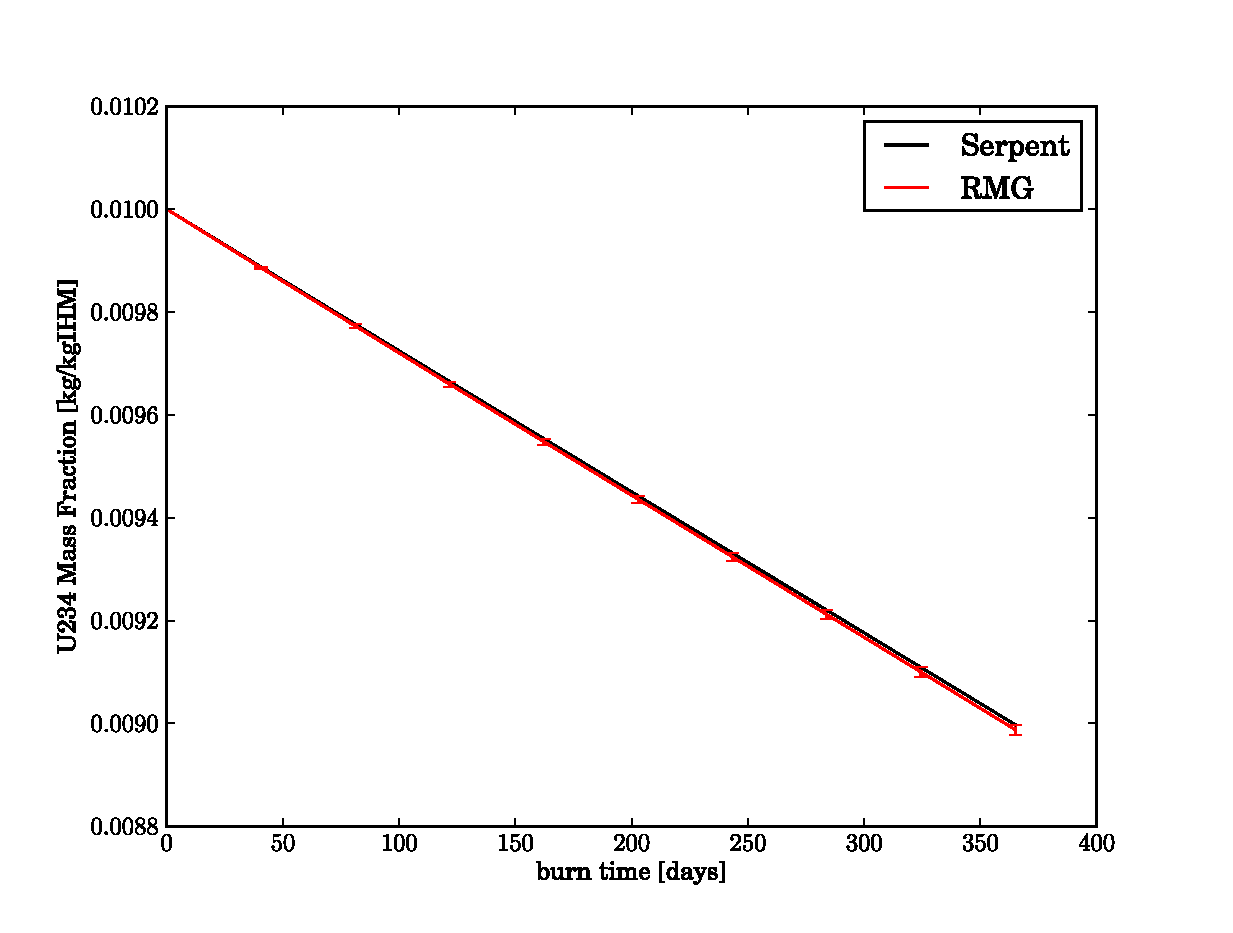
\includegraphics[scale=0.3]{multigroup_method/figs/benchmark/U234_Mass_Fraction_.eps}
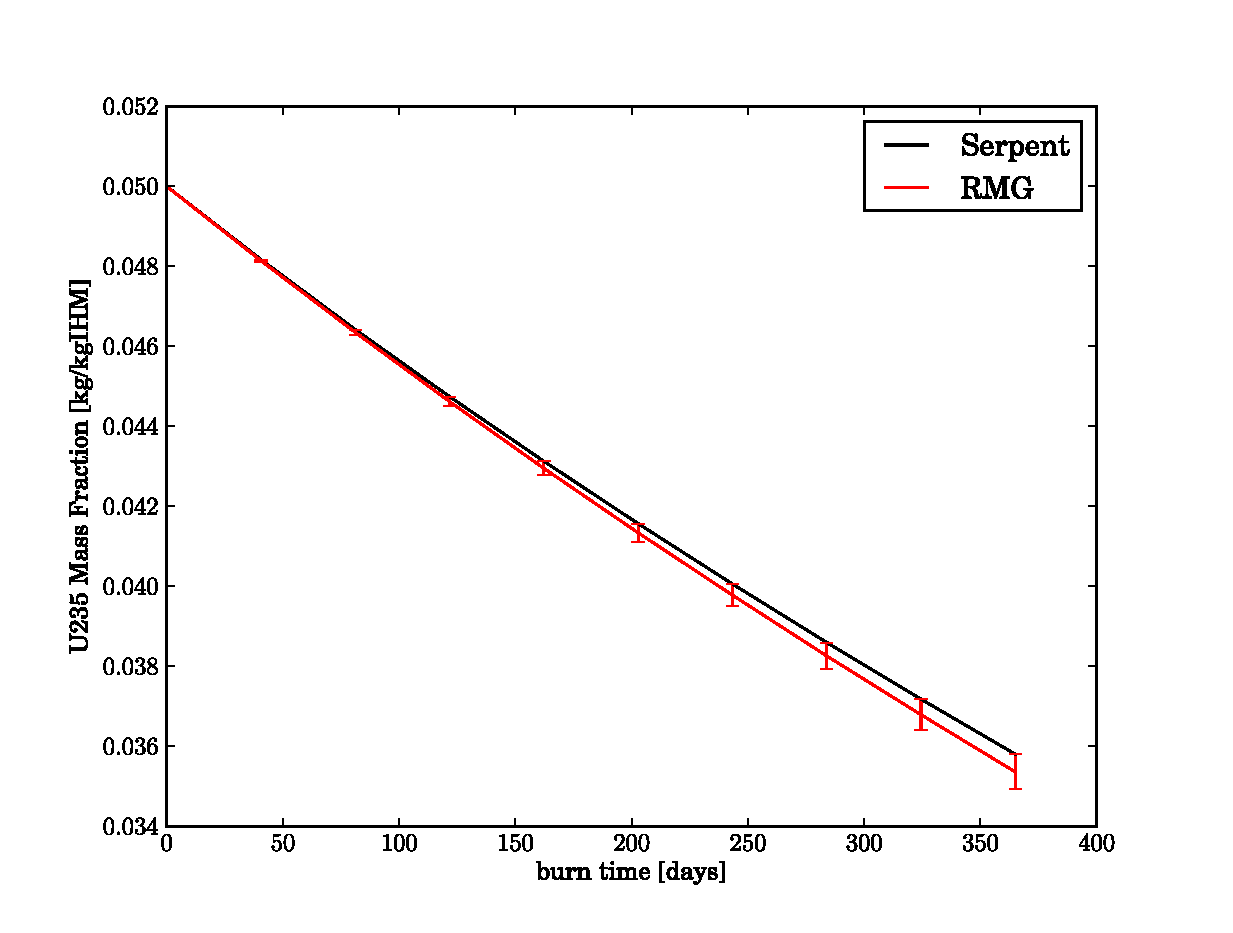
\includegraphics[scale=0.3]{multigroup_method/figs/benchmark/U235_Mass_Fraction_.eps}
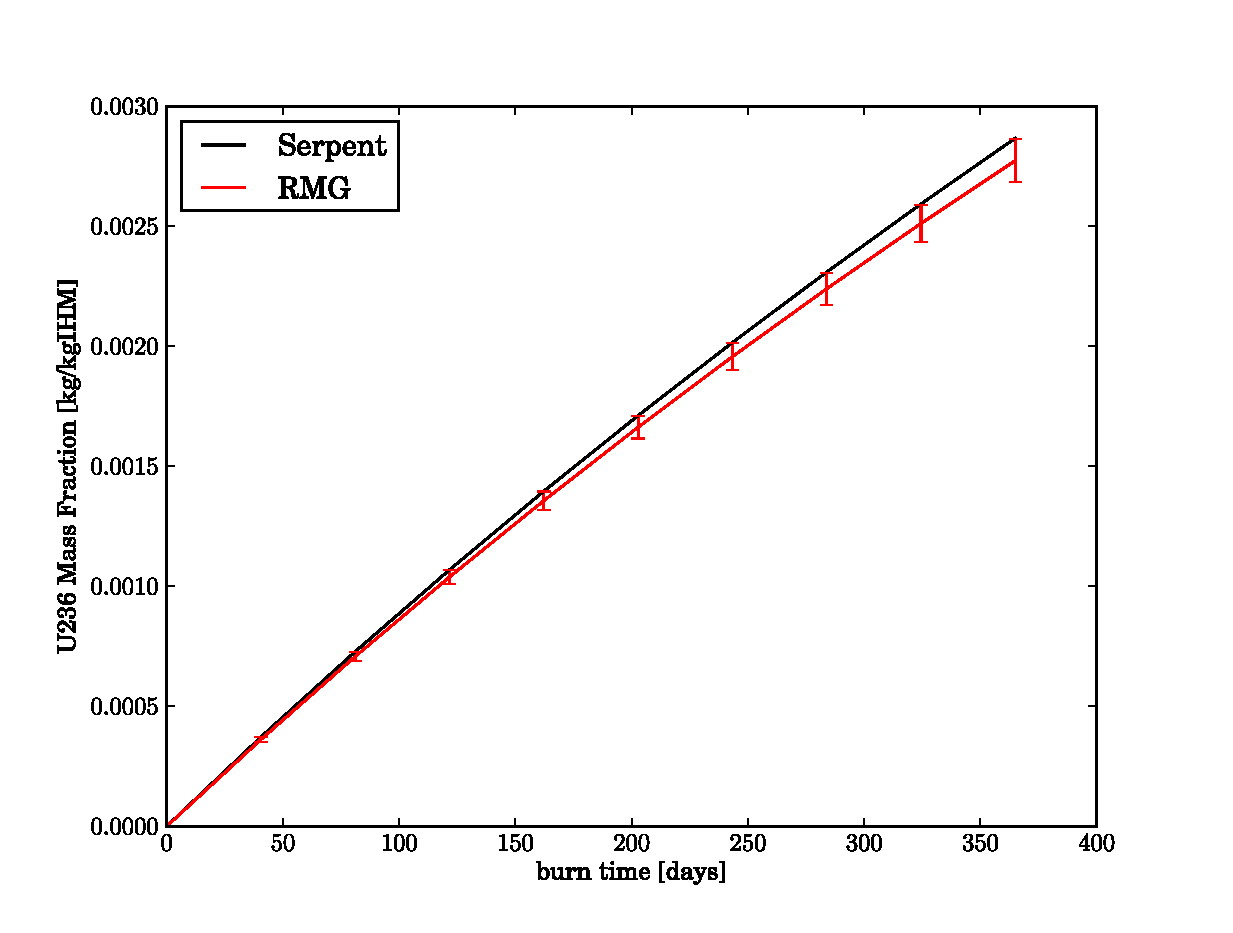
\includegraphics[scale=0.3]{multigroup_method/figs/benchmark/U236_Mass_Fraction_.eps}
\includegraphics[scale=0.3]{multigroup_method/figs/benchmark/U238_Mass_Fraction_.eps}
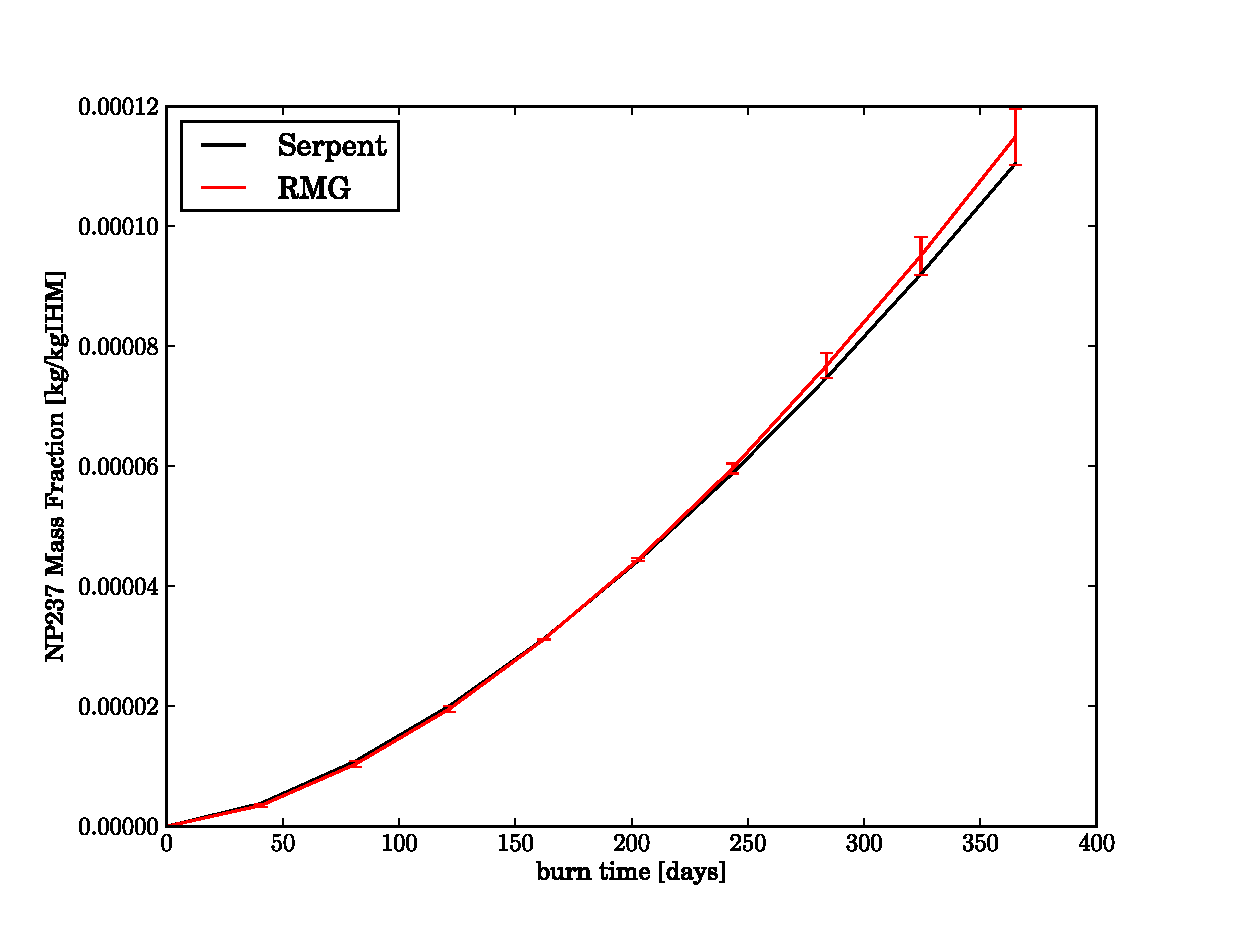
\includegraphics[scale=0.3]{multigroup_method/figs/benchmark/NP237_Mass_Fraction_.eps}
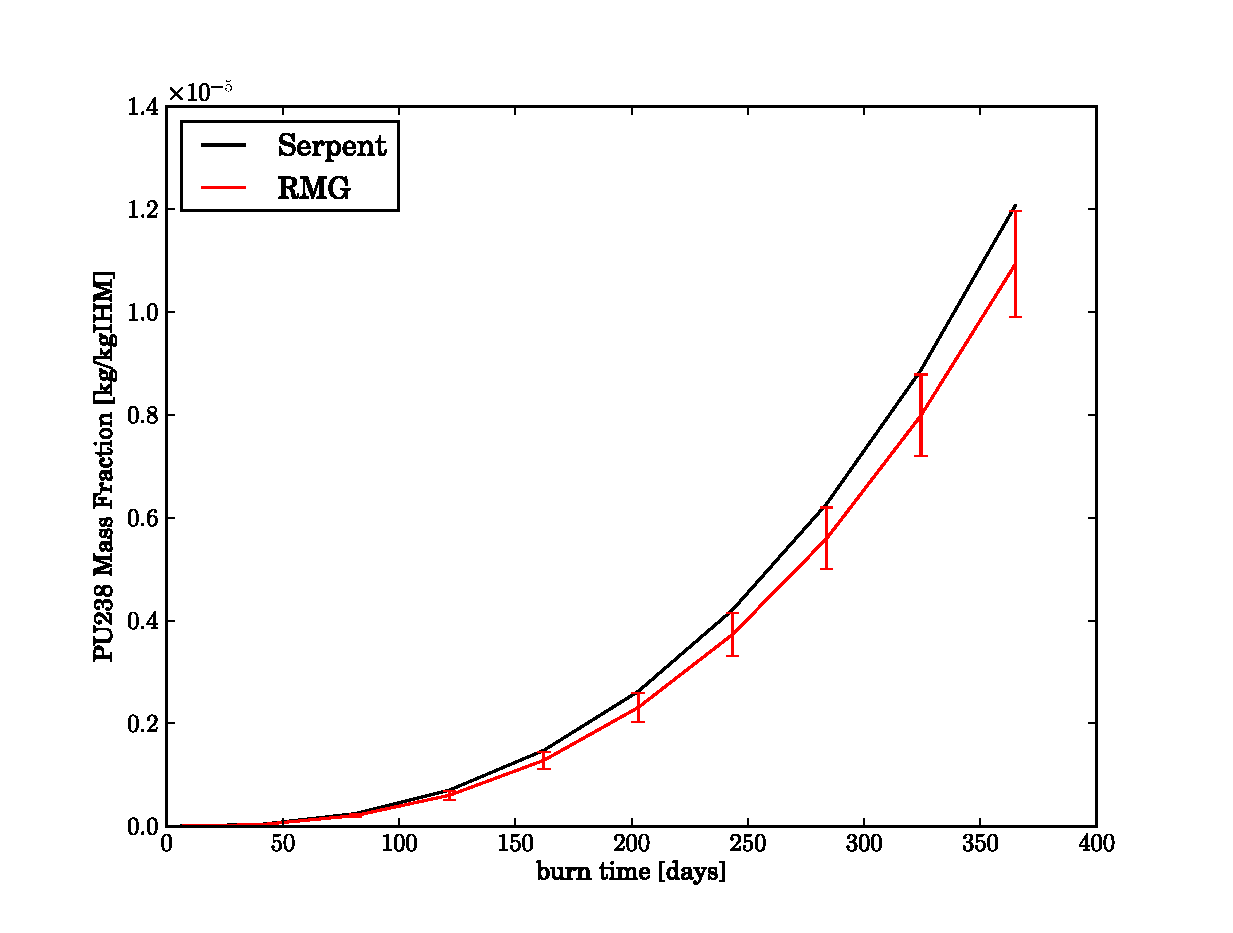
\includegraphics[scale=0.3]{multigroup_method/figs/benchmark/PU238_Mass_Fraction_.eps}
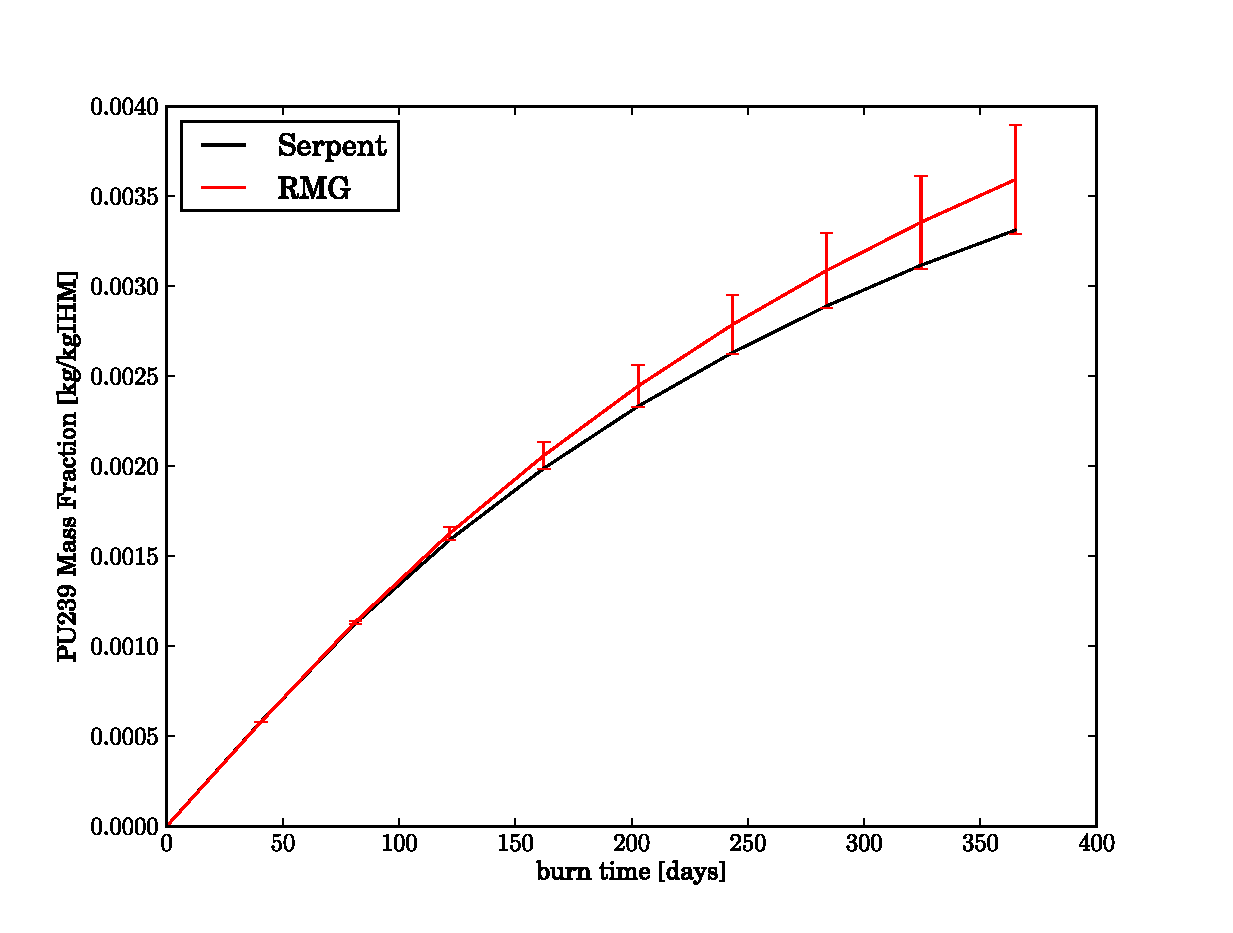
\includegraphics[scale=0.3]{multigroup_method/figs/benchmark/PU239_Mass_Fraction_.eps}
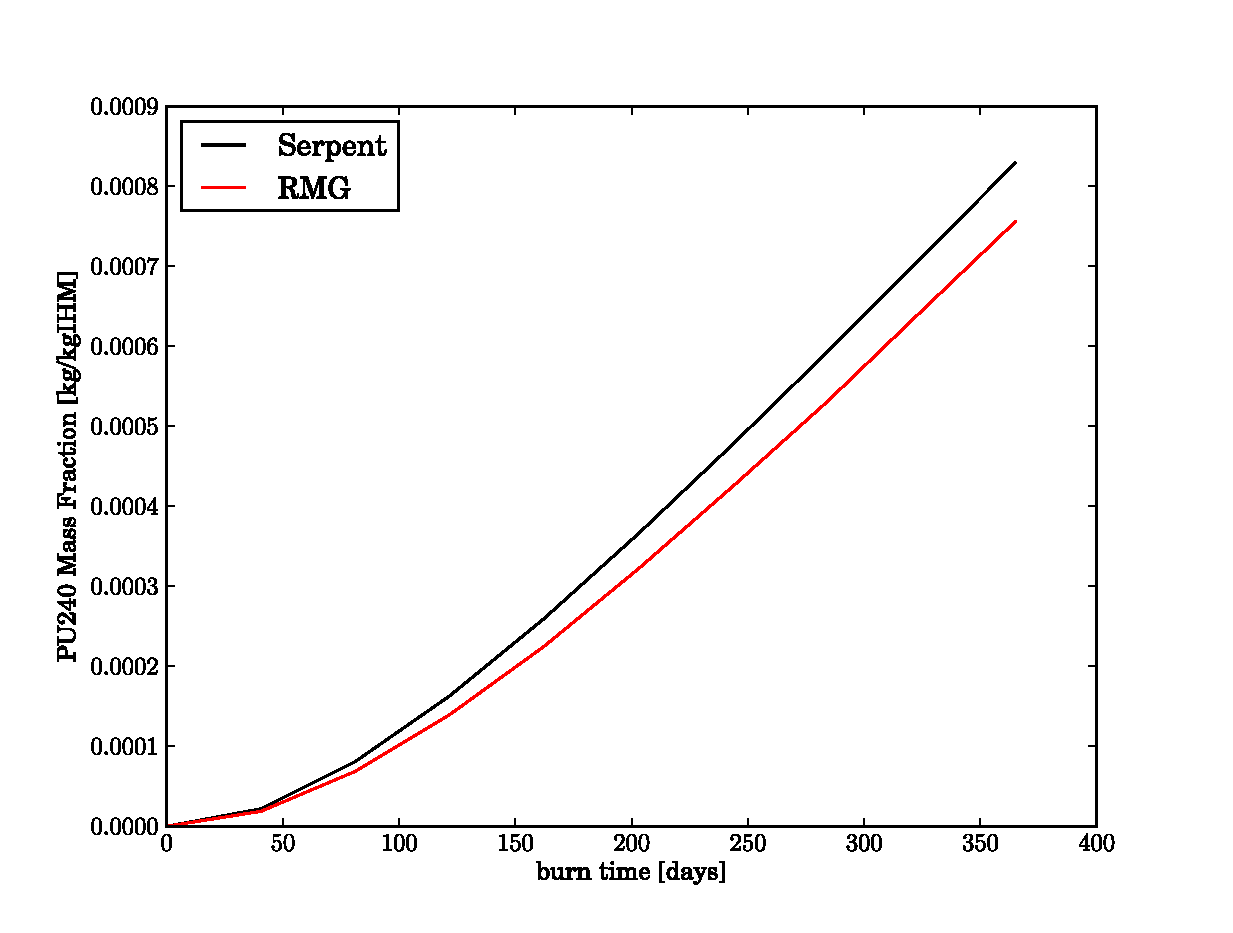
\includegraphics[scale=0.3]{multigroup_method/figs/benchmark/PU240_Mass_Fraction_.eps}
\end{center}
\end{figure}
\begin{figure}[htbp]
\caption{Actinide Mass Fraction Benchmarks (Cont.)}
\label{act_benchmark_cont}
\begin{center}
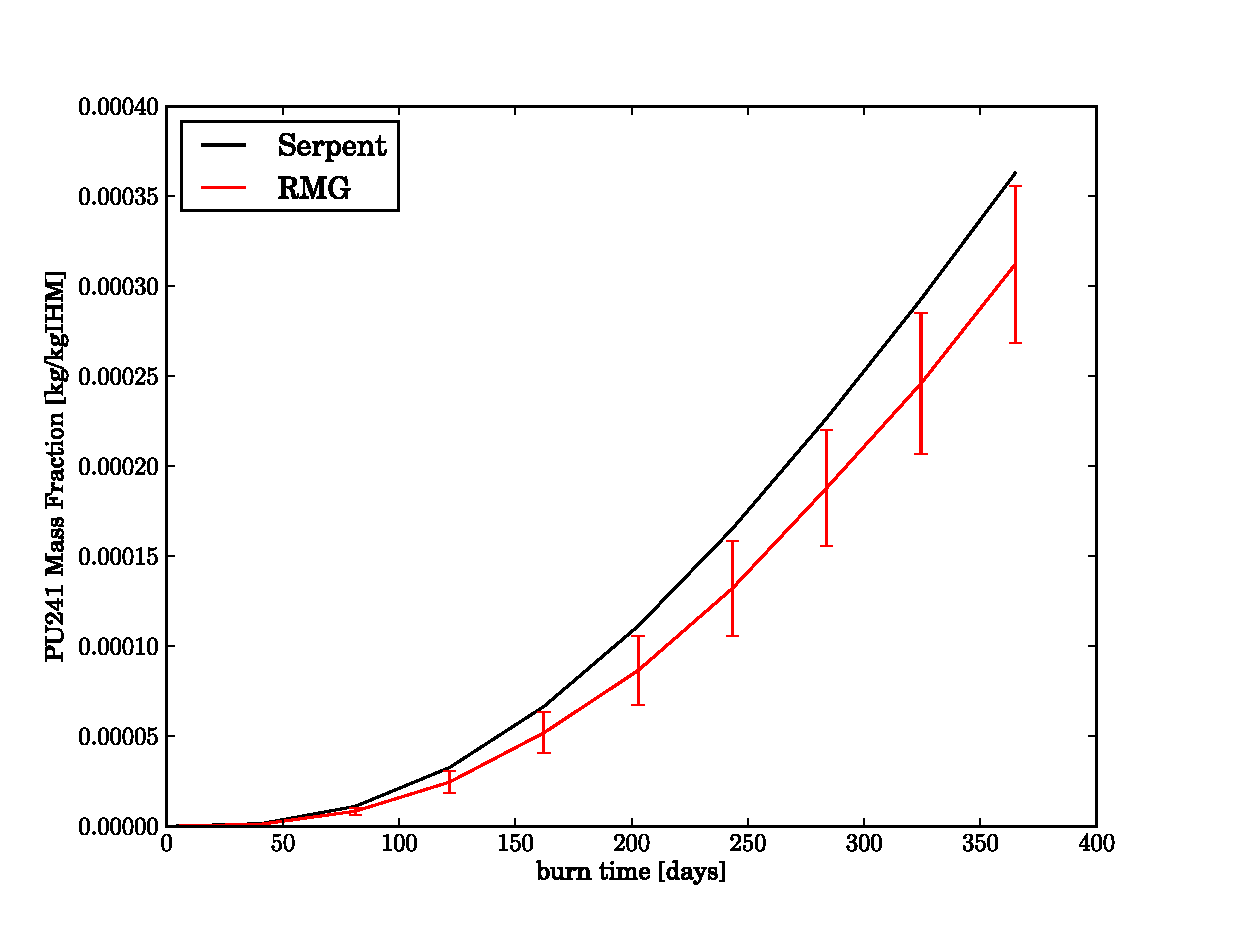
\includegraphics[scale=0.3]{multigroup_method/figs/benchmark/PU241_Mass_Fraction_.eps}
\includegraphics[scale=0.3]{multigroup_method/figs/benchmark/PU242_Mass_Fraction_.eps}
\includegraphics[scale=0.3]{multigroup_method/figs/benchmark/AM241_Mass_Fraction_.eps}
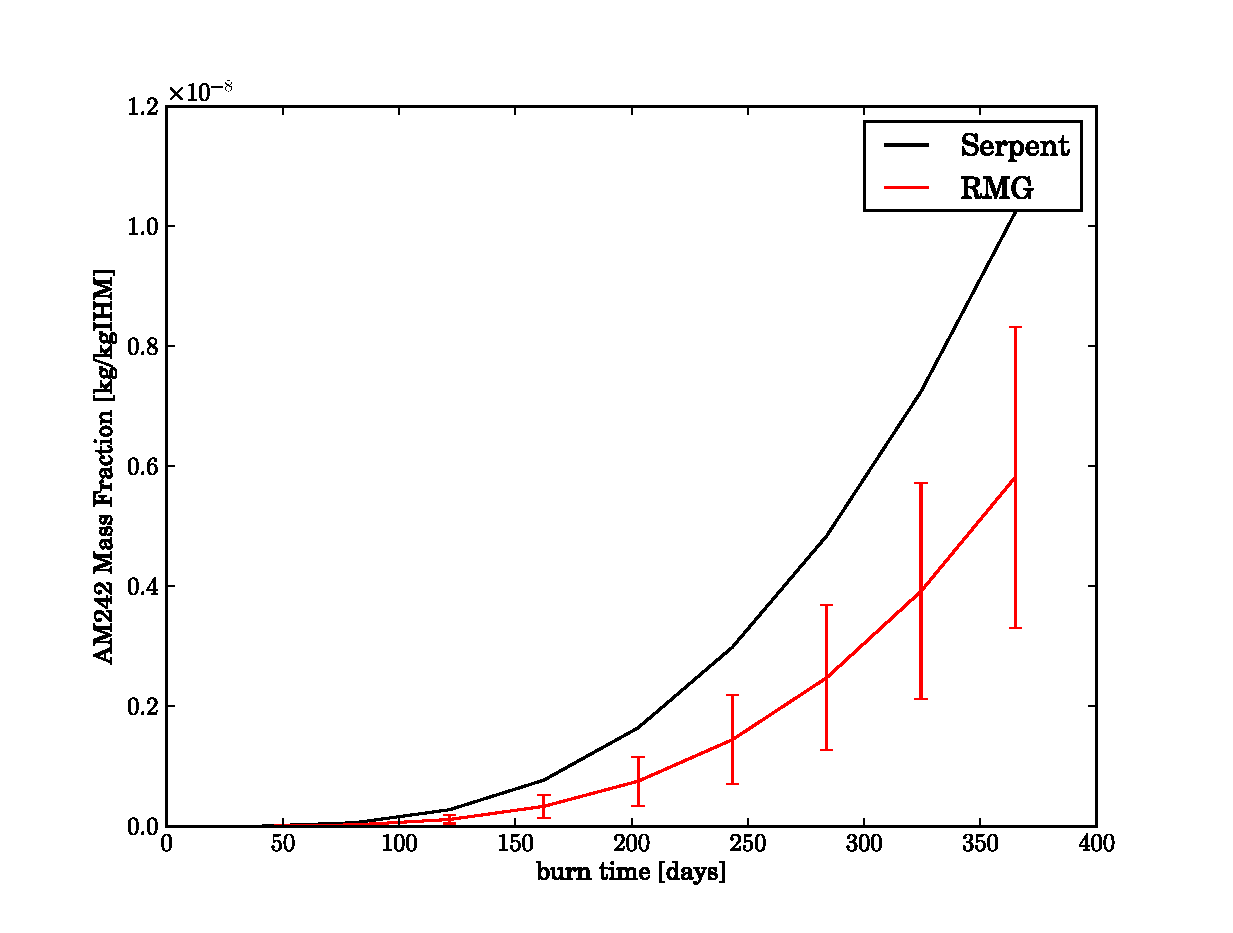
\includegraphics[scale=0.3]{multigroup_method/figs/benchmark/AM242_Mass_Fraction_.eps}
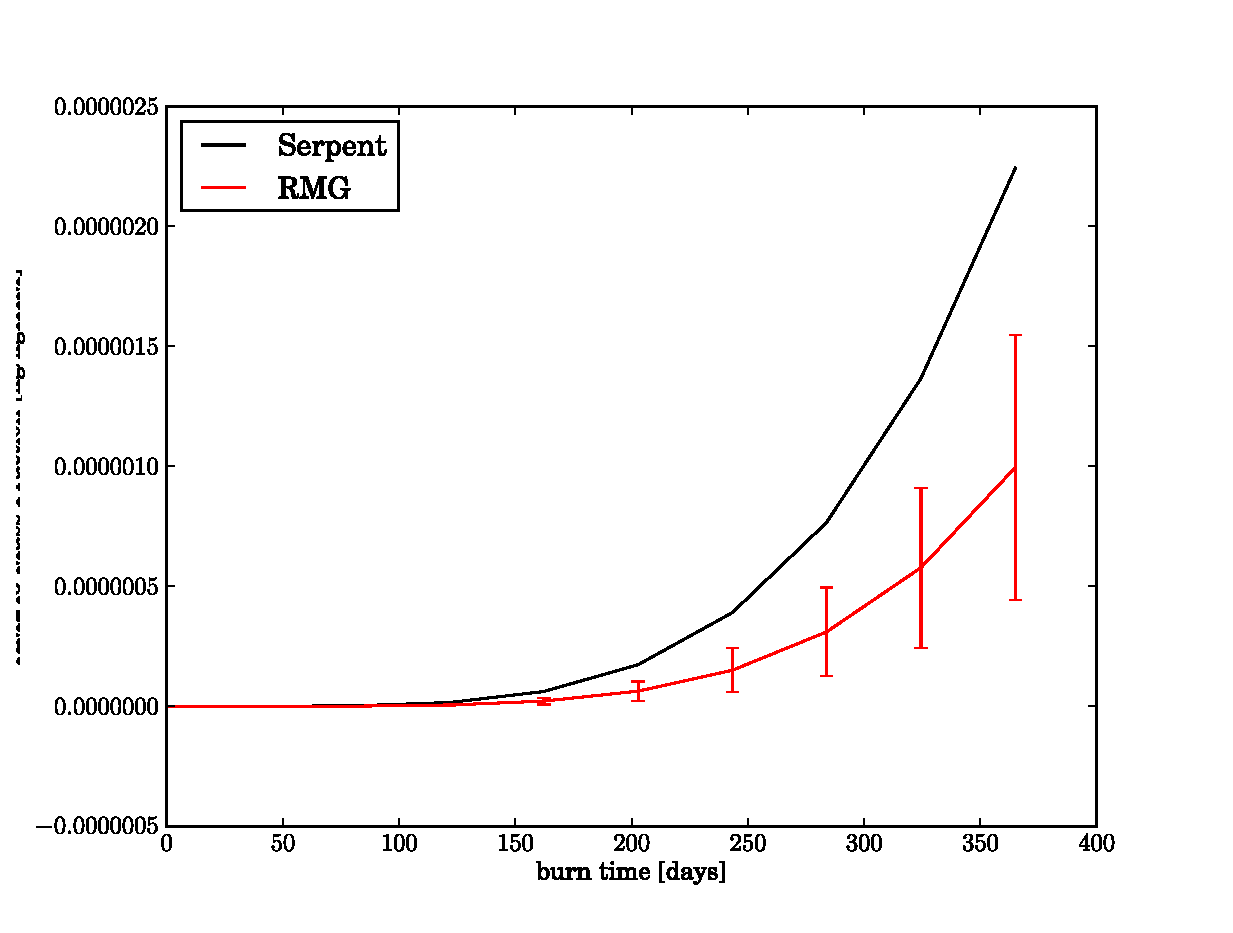
\includegraphics[scale=0.3]{multigroup_method/figs/benchmark/AM243_Mass_Fraction_.eps}
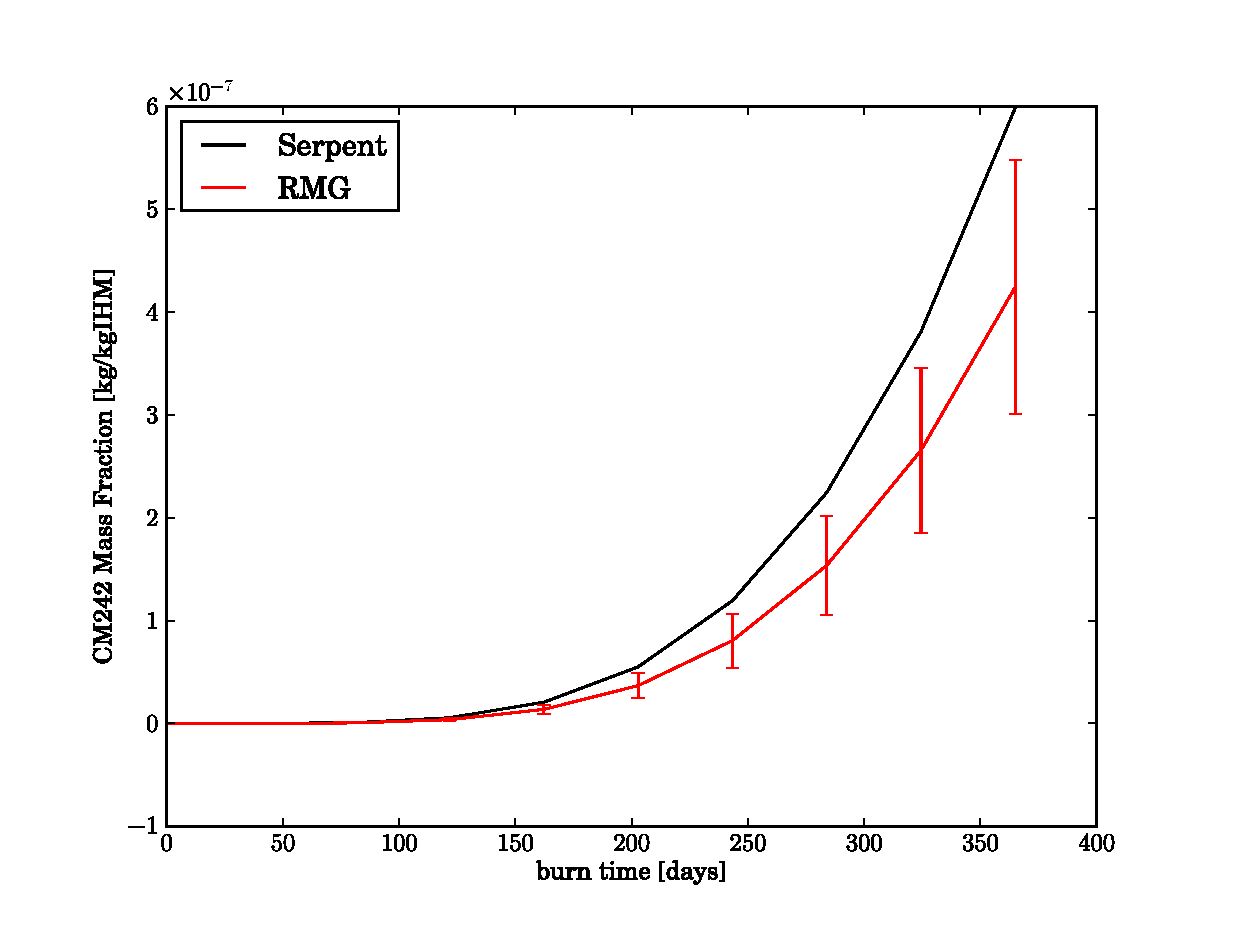
\includegraphics[scale=0.3]{multigroup_method/figs/benchmark/CM242_Mass_Fraction_.eps}
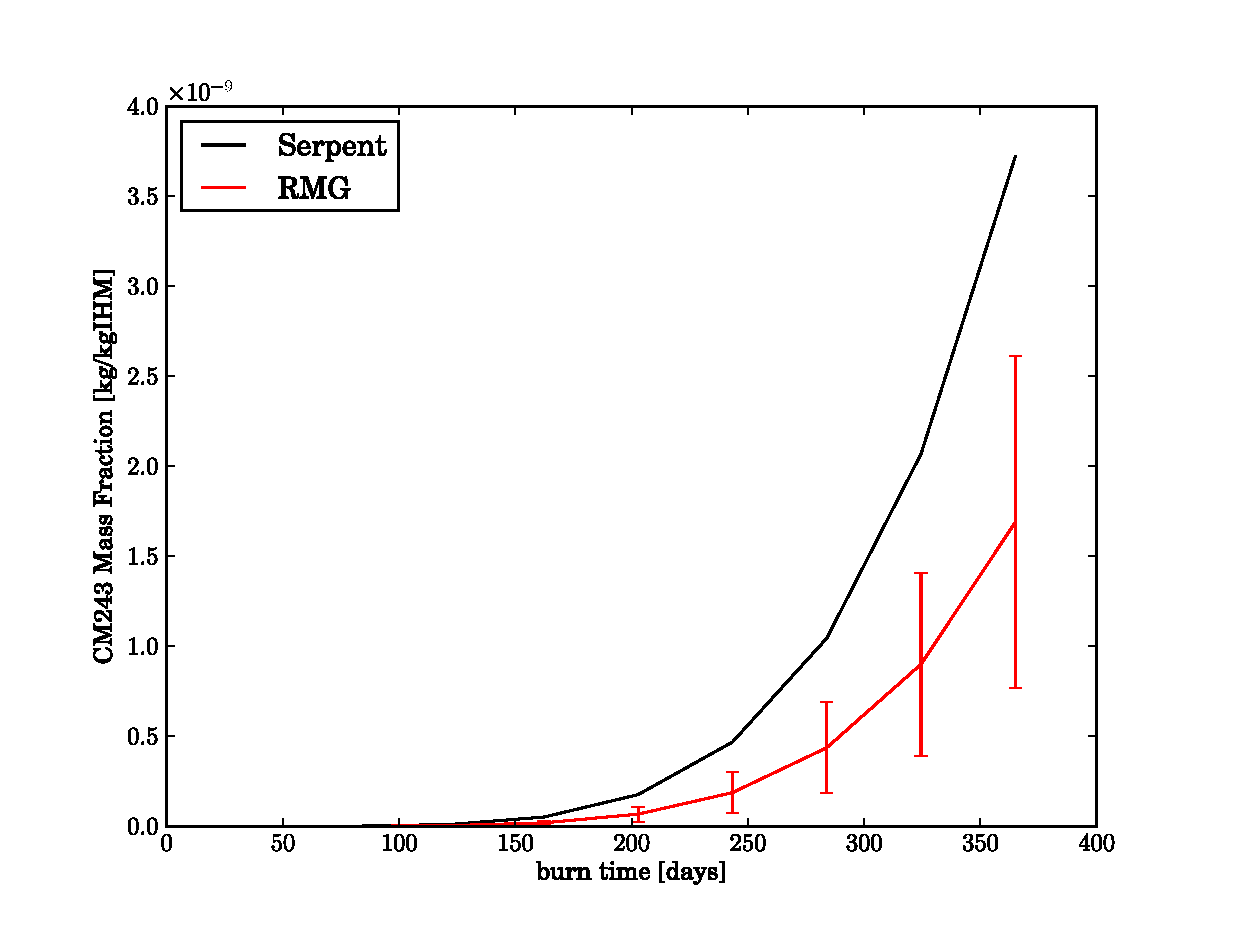
\includegraphics[scale=0.3]{multigroup_method/figs/benchmark/CM243_Mass_Fraction_.eps}
\includegraphics[scale=0.3]{multigroup_method/figs/benchmark/CM244_Mass_Fraction_.eps}
\end{center}
\end{figure}
\begin{figure}[htbp]
\caption{Actinide \& Fission Product Mass Fraction Benchmarks}
\label{act_fp_benchmark}
\begin{center}
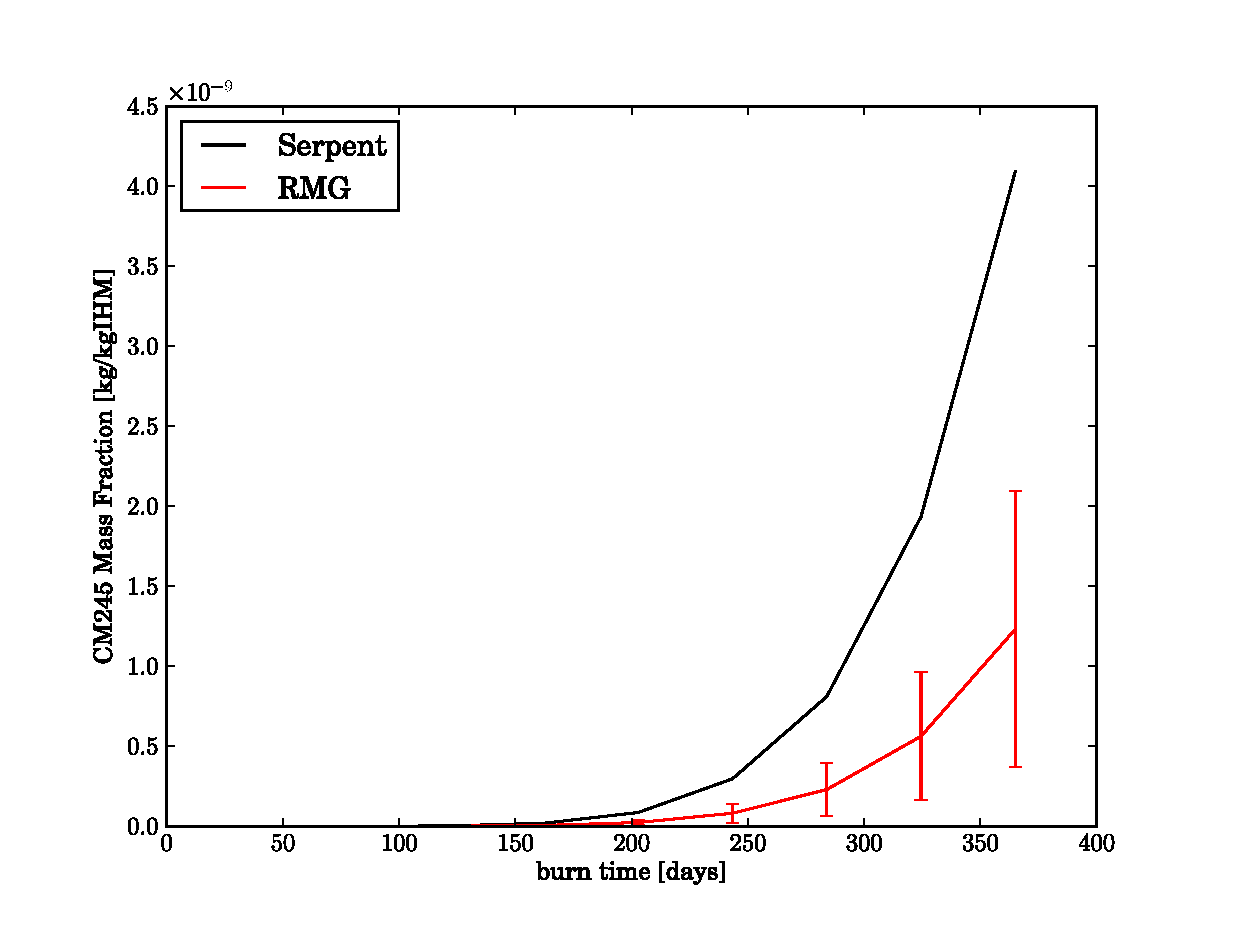
\includegraphics[scale=0.3]{multigroup_method/figs/benchmark/CM245_Mass_Fraction_.eps}
\includegraphics[scale=0.3]{multigroup_method/figs/benchmark/CM246_Mass_Fraction_.eps}
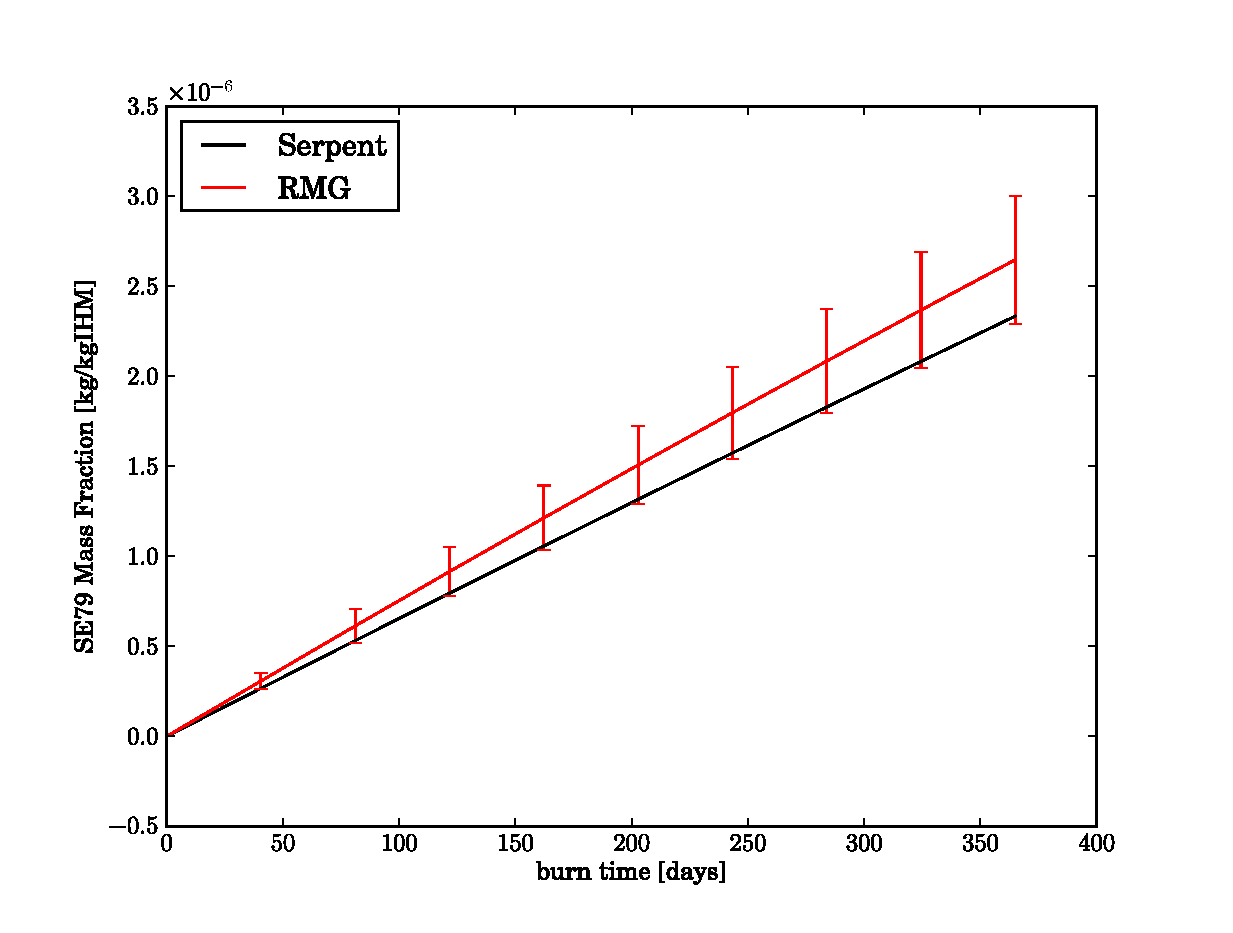
\includegraphics[scale=0.3]{multigroup_method/figs/benchmark/SE79_Mass_Fraction_.eps}
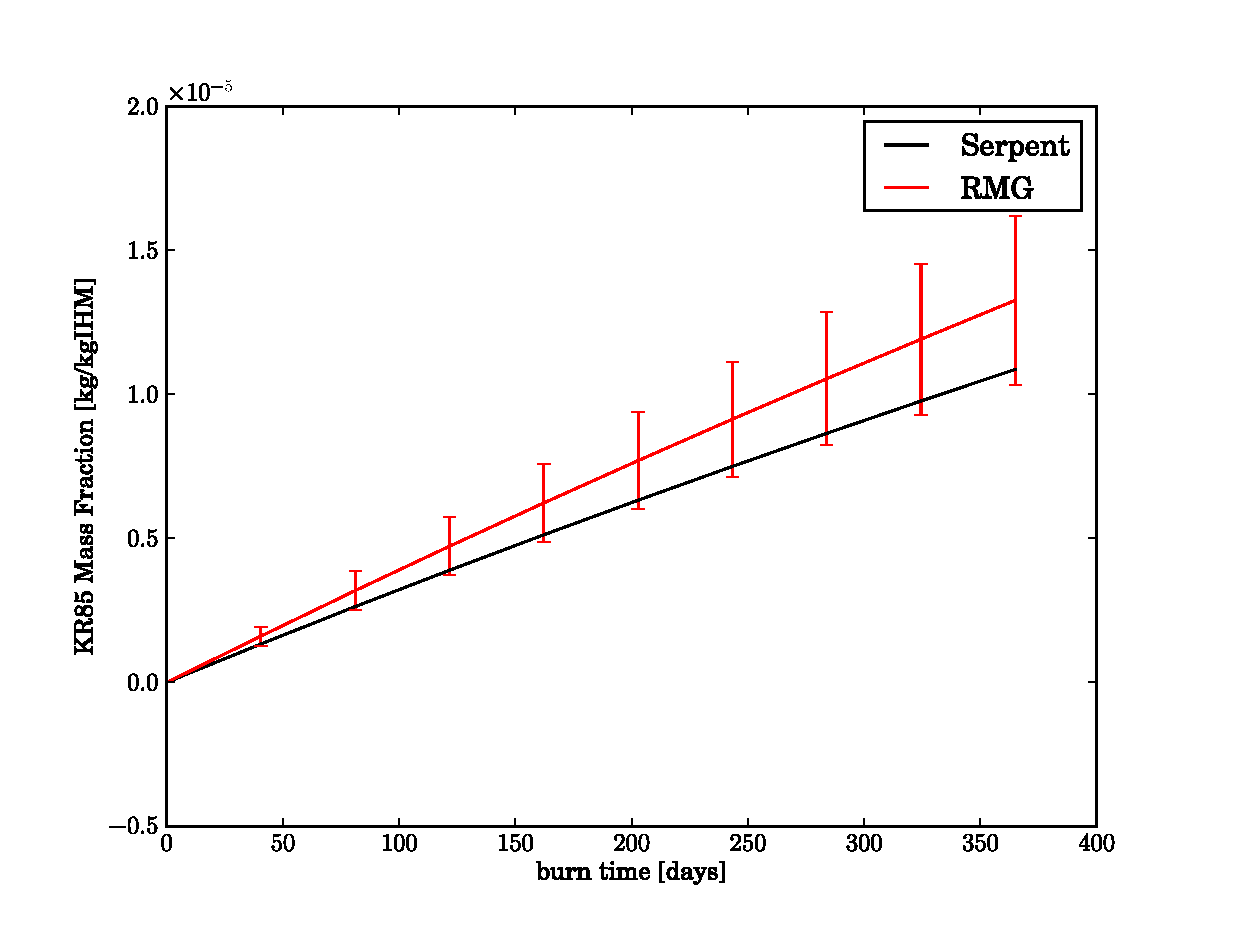
\includegraphics[scale=0.3]{multigroup_method/figs/benchmark/KR85_Mass_Fraction_.eps}
\includegraphics[scale=0.3]{multigroup_method/figs/benchmark/SR90_Mass_Fraction_.eps}
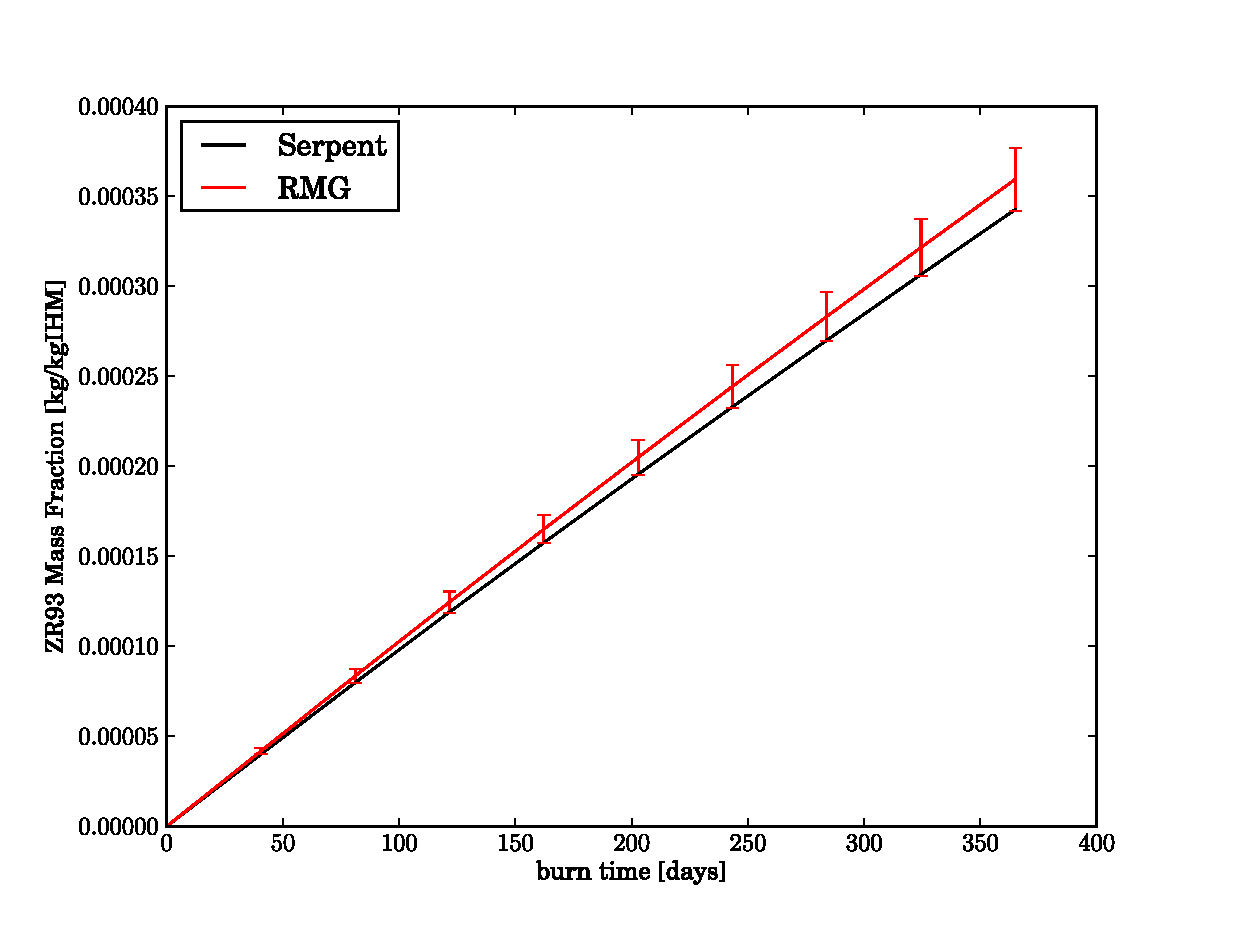
\includegraphics[scale=0.3]{multigroup_method/figs/benchmark/ZR93_Mass_Fraction_.eps}
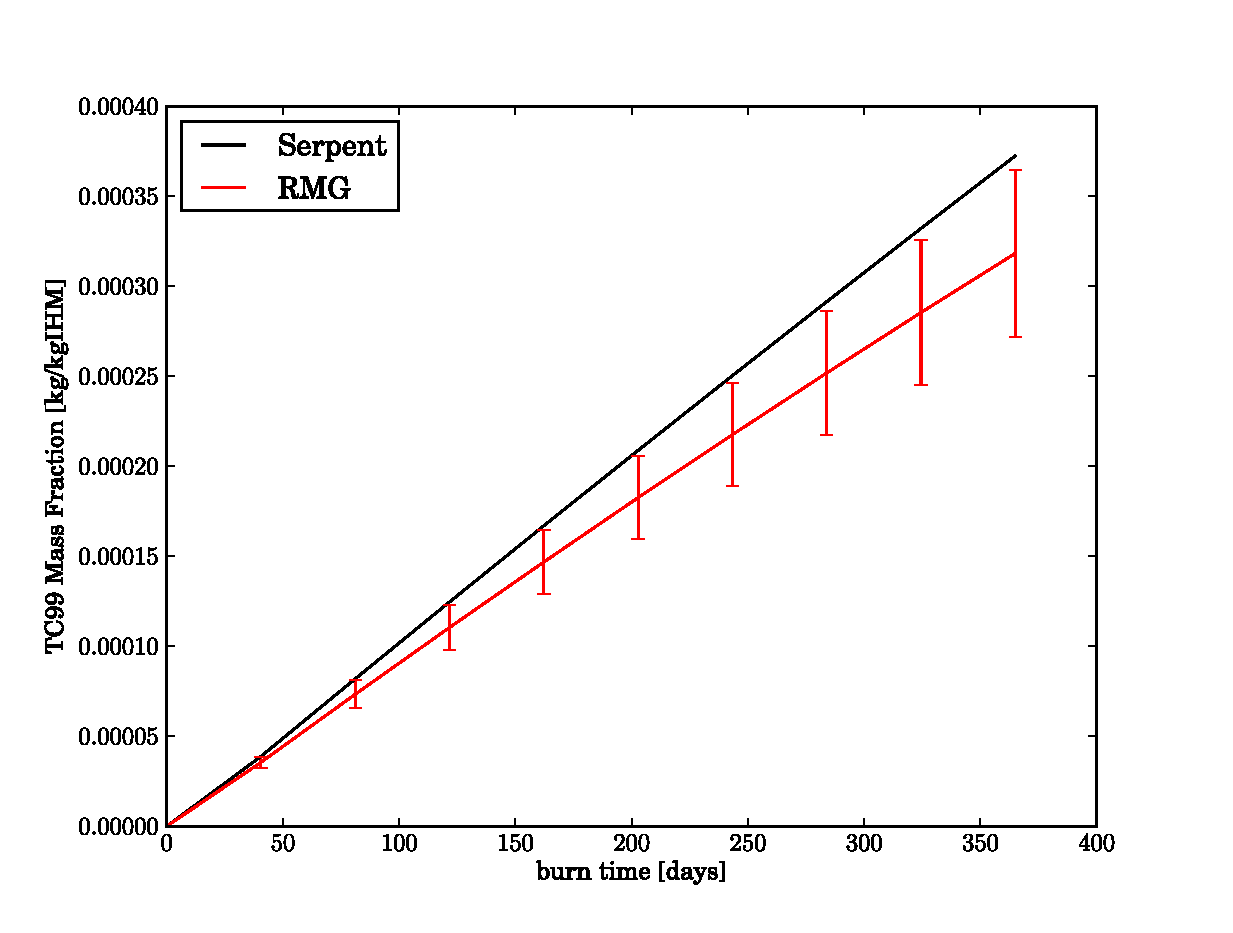
\includegraphics[scale=0.3]{multigroup_method/figs/benchmark/TC99_Mass_Fraction_.eps}
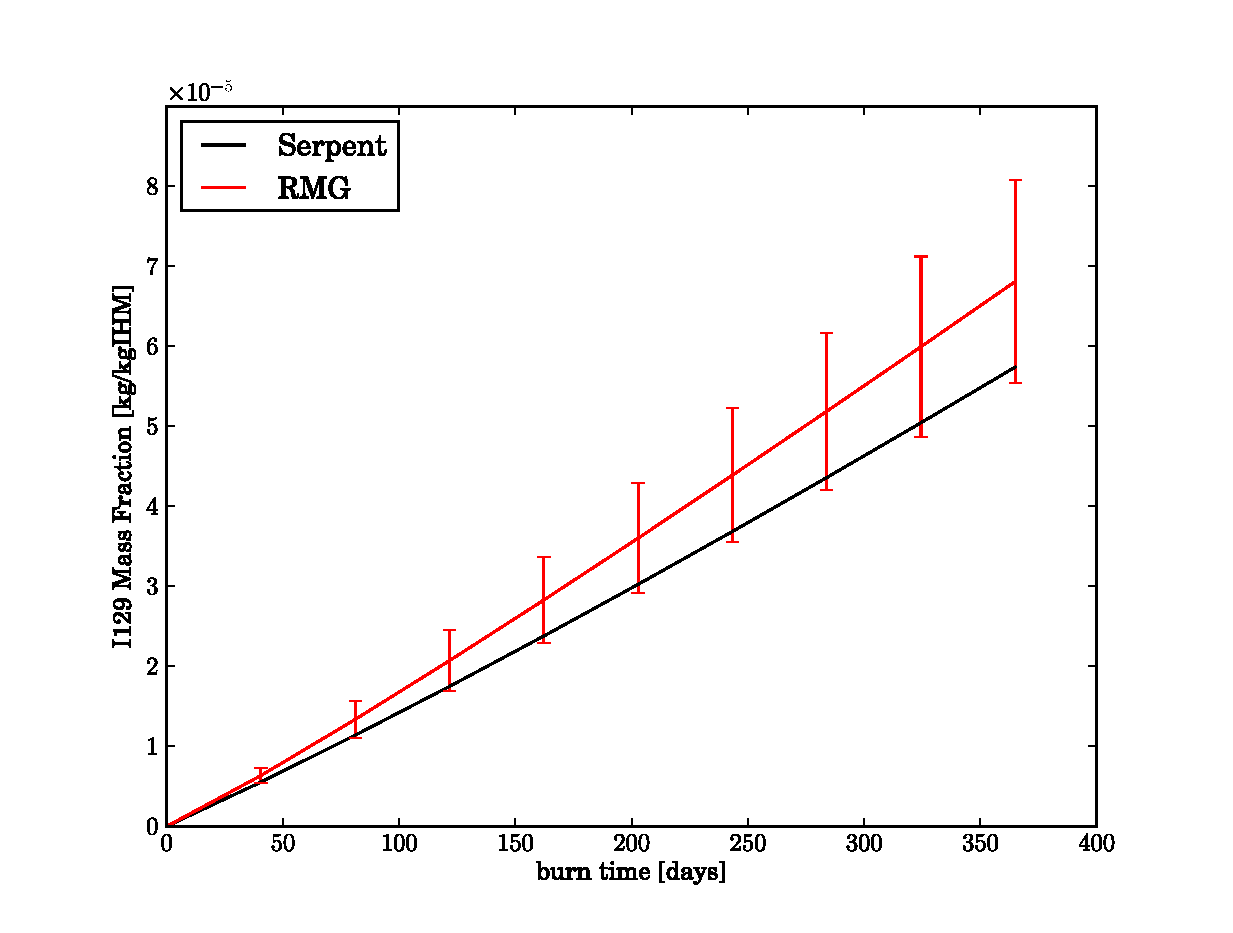
\includegraphics[scale=0.3]{multigroup_method/figs/benchmark/I129_Mass_Fraction_.eps}
\end{center}
\end{figure}
\begin{figure}[htbp]
\caption{Fission Product Mass Fraction Benchmarks}
\label{fp_benchmark}
\begin{center}
\includegraphics[scale=0.3]{multigroup_method/figs/benchmark/PD107_Mass_Fraction_.eps}
\includegraphics[scale=0.3]{multigroup_method/figs/benchmark/CS134_Mass_Fraction_.eps}
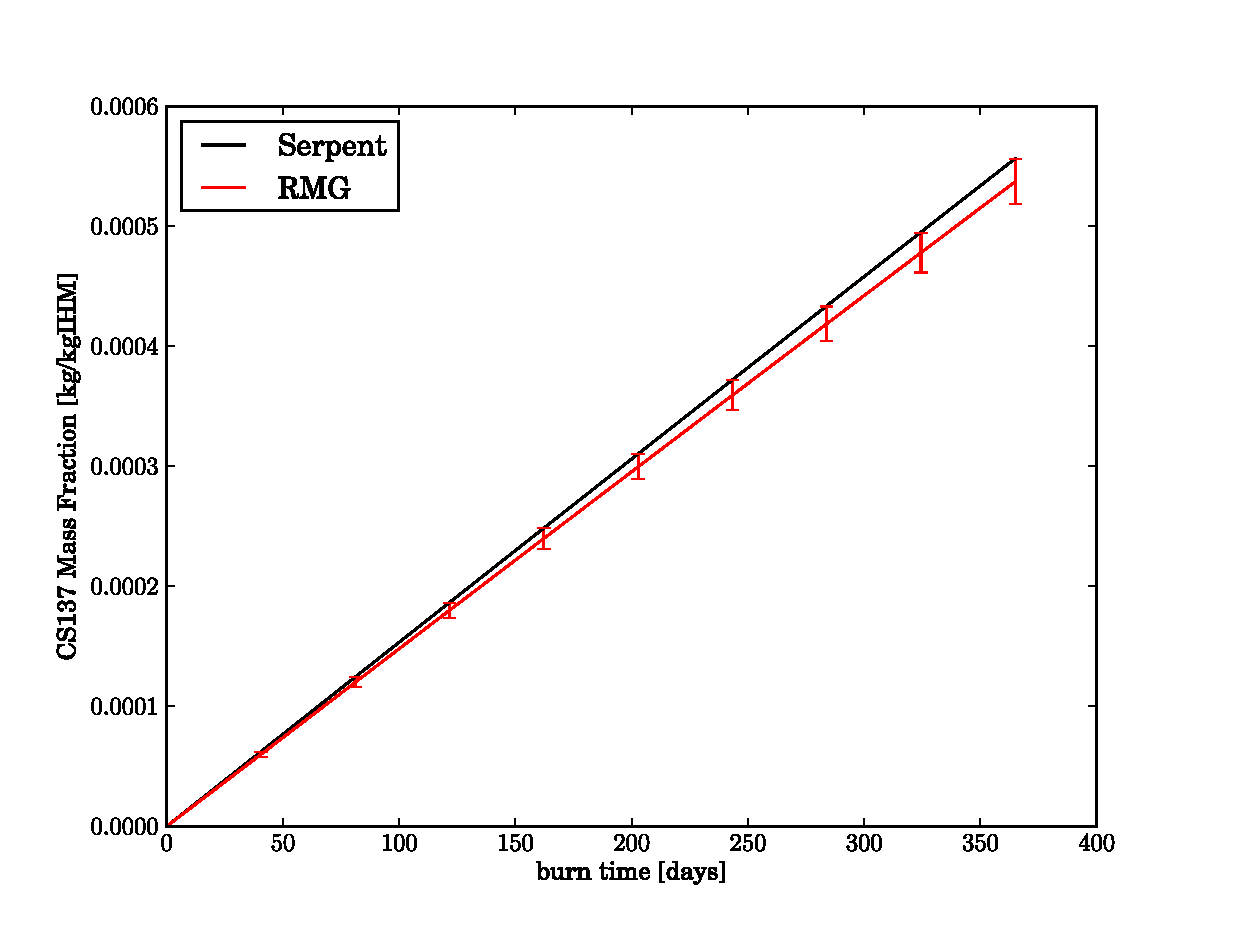
\includegraphics[scale=0.3]{multigroup_method/figs/benchmark/CS137_Mass_Fraction_.eps}
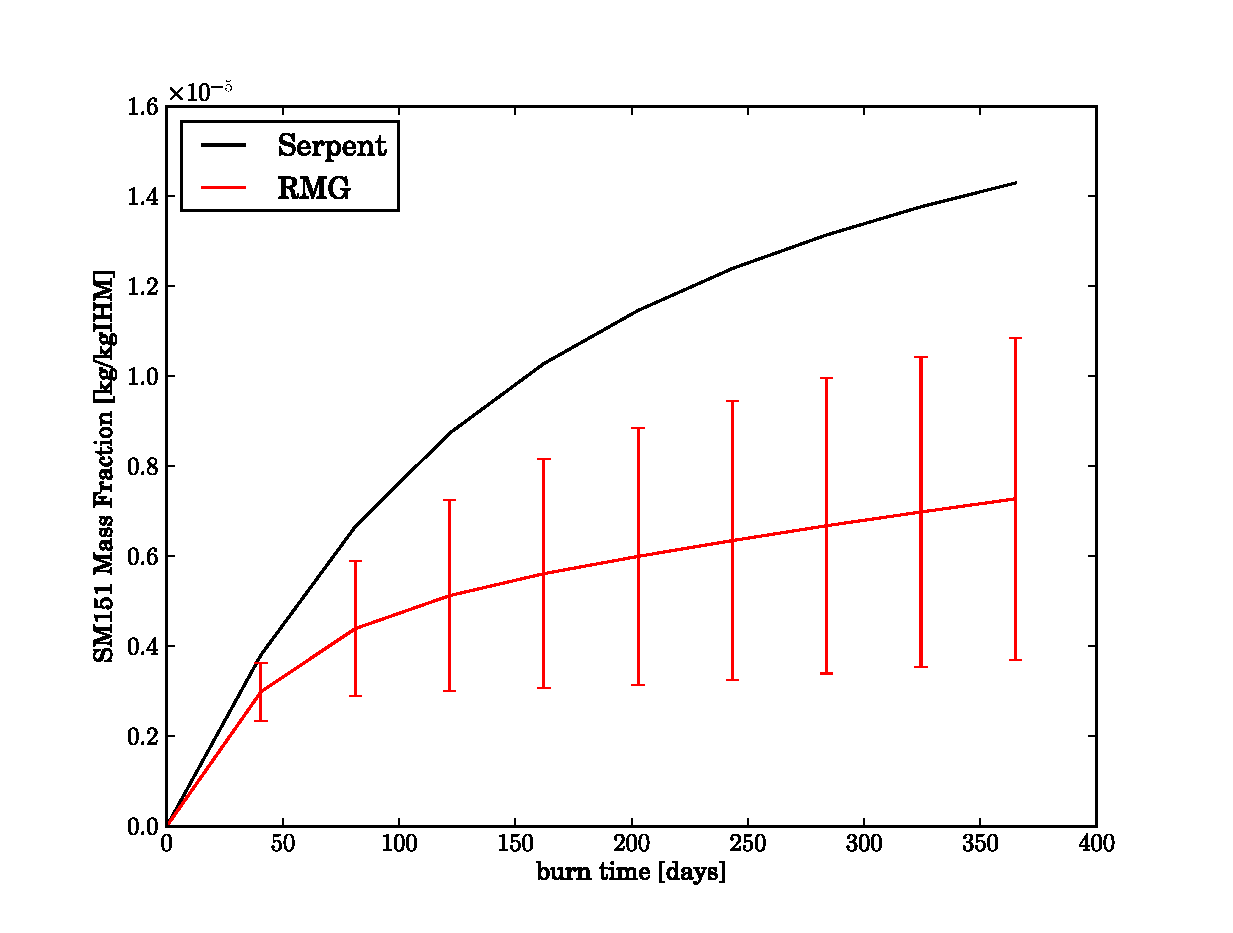
\includegraphics[scale=0.3]{multigroup_method/figs/benchmark/SM151_Mass_Fraction_.eps}
\end{center}
\end{figure}


As is seen in these figures, there is good agrement between the transmutation vectors computed by
Serpent and those computed by the RMG via Origen.  The instances with non-trivial disagreements are 
largely in the higher order actinides.  These nuclides exist in such small amounts, that the relatively
high errors do not adeversely effect the neutronic performance of the fuel.

However, the true strength of the RMG methodology is 
that it takes into account the time evolotion of the cross sections as well.  For the same set 
of nuclides above, Figures \ref{act_xs_benchmark}-\ref{fp_xs_benchmark} display total, absorption,
scattering and fission one-group cross sections as a function of burn time.  One-group cross sections 
are used here in favor of the multigroup cross sections because they capture the total differences 
between data sets while removing the complexity of plotting three dimensional information.

\begin{figure}[htbp]
\caption{Actinide One-Group Cross-Section Benchmarks}
\label{act_xs_benchmark}
\begin{center}
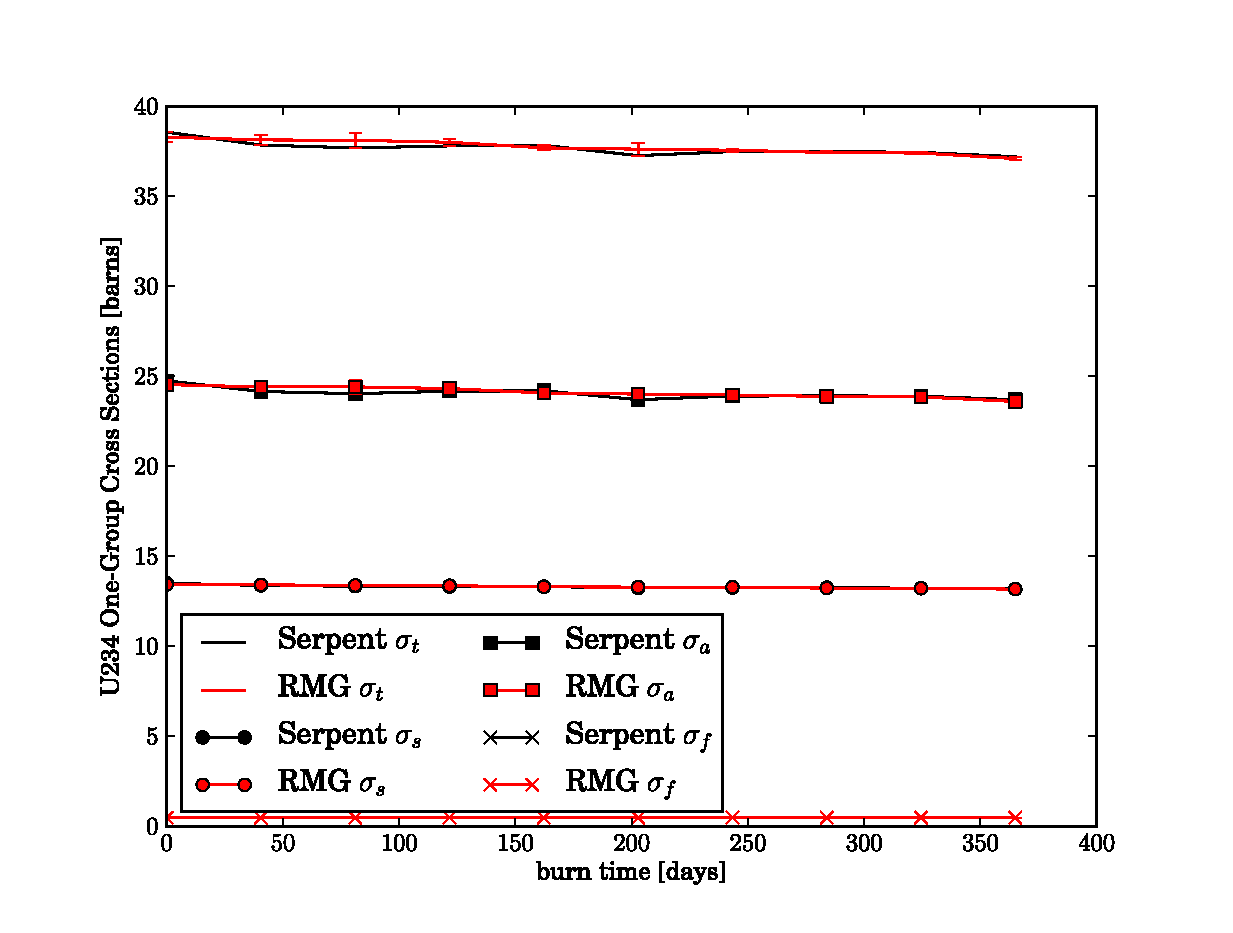
\includegraphics[scale=0.3]{multigroup_method/figs/benchmark/U234_1g_xs.eps}
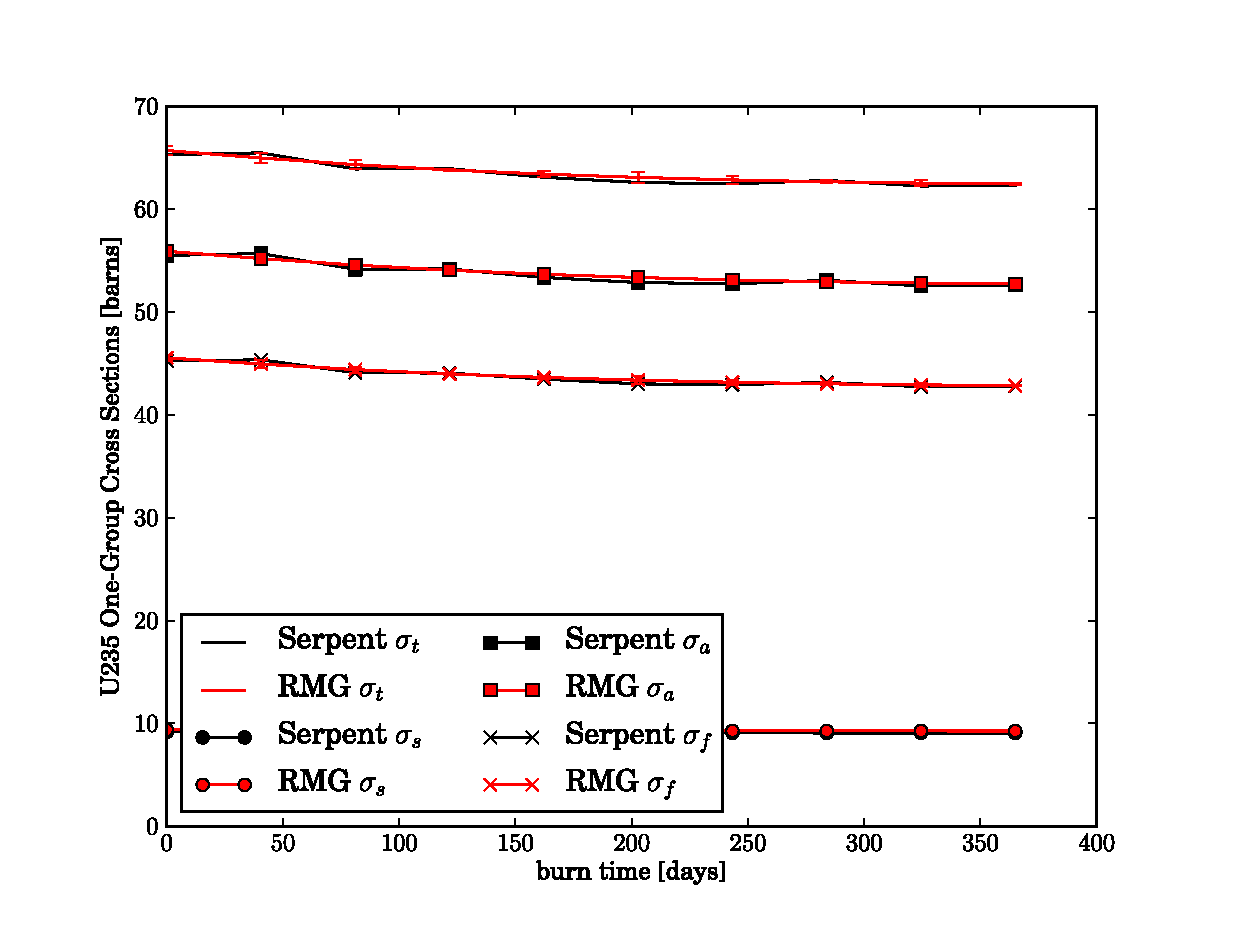
\includegraphics[scale=0.3]{multigroup_method/figs/benchmark/U235_1g_xs.eps}
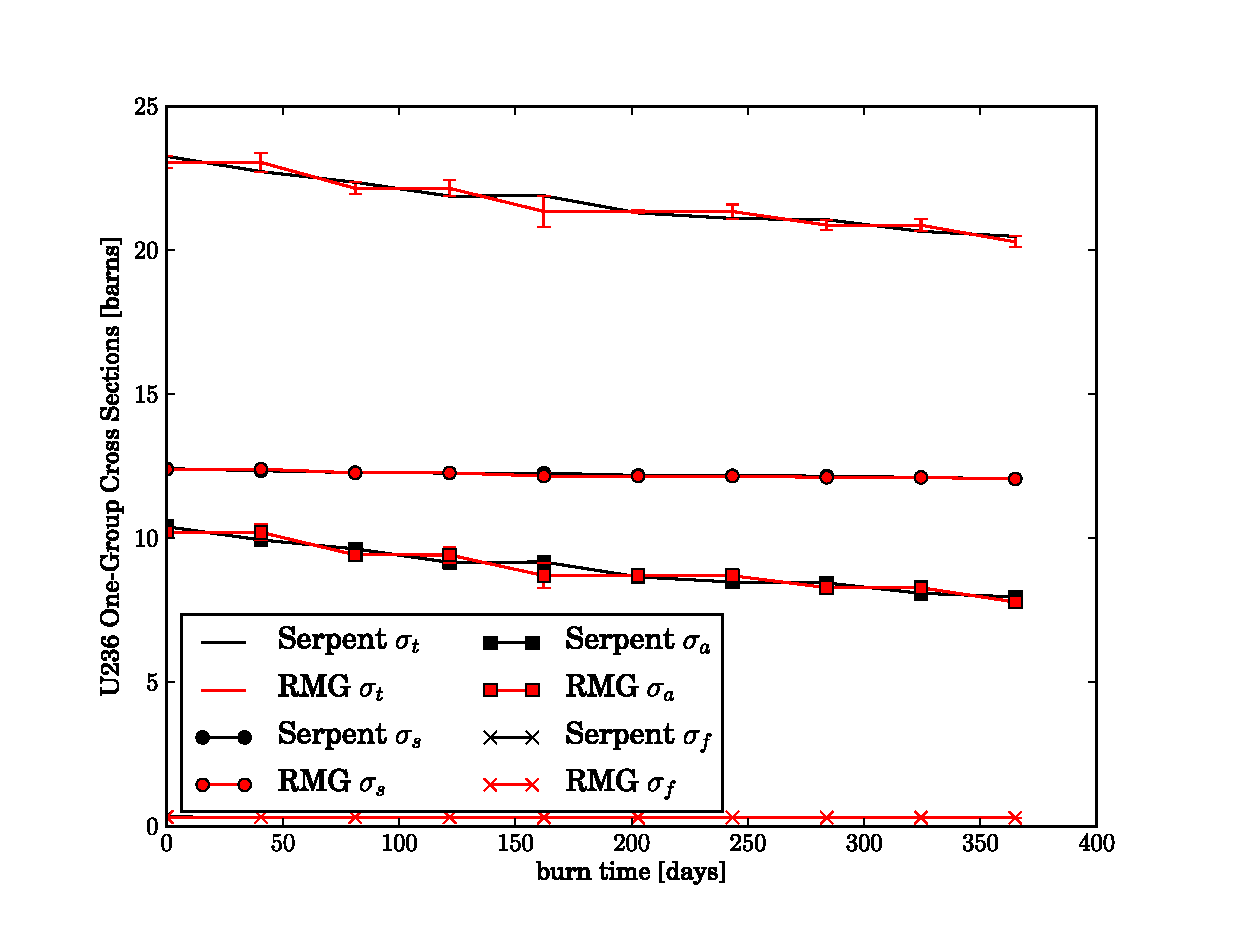
\includegraphics[scale=0.3]{multigroup_method/figs/benchmark/U236_1g_xs.eps}
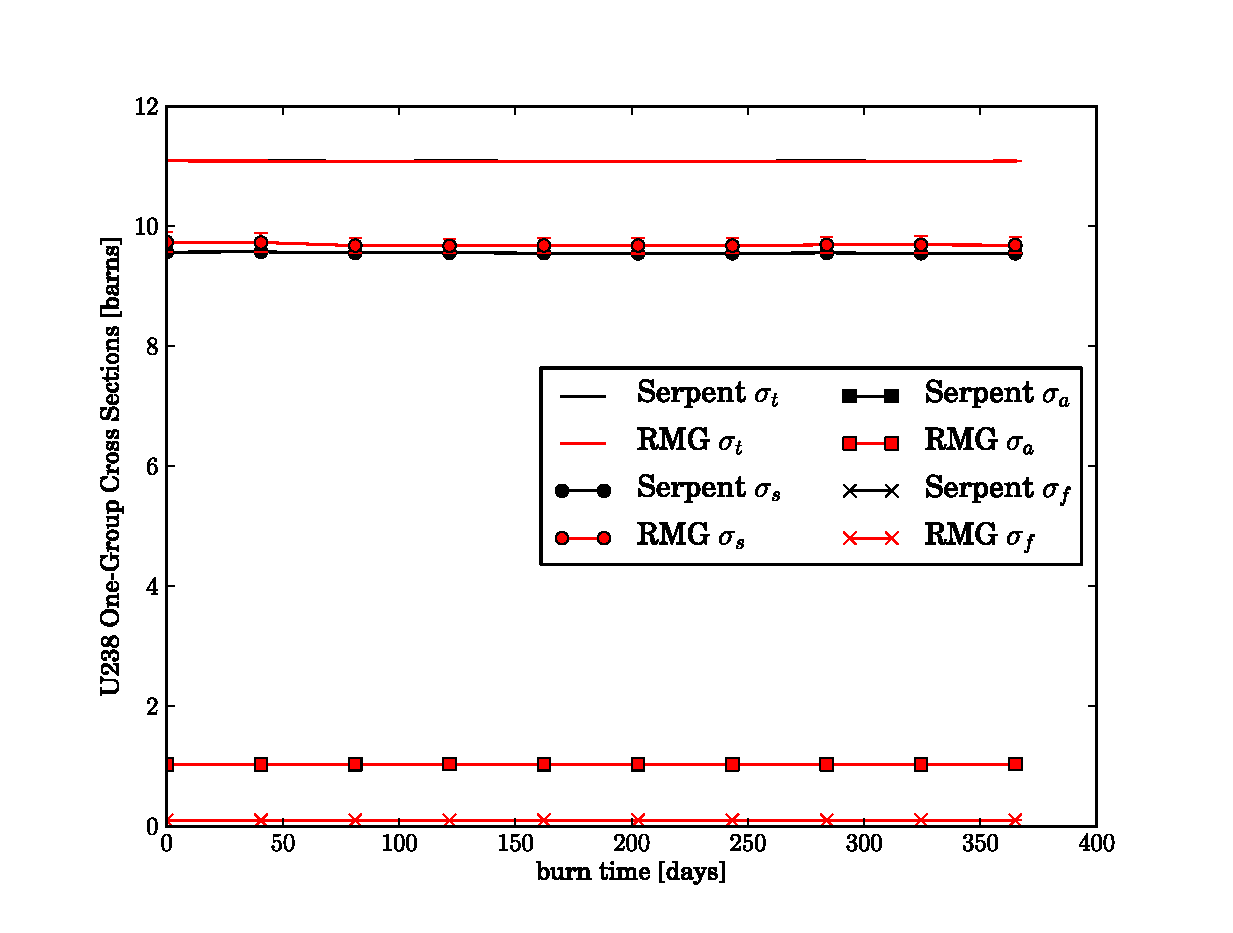
\includegraphics[scale=0.3]{multigroup_method/figs/benchmark/U238_1g_xs.eps}
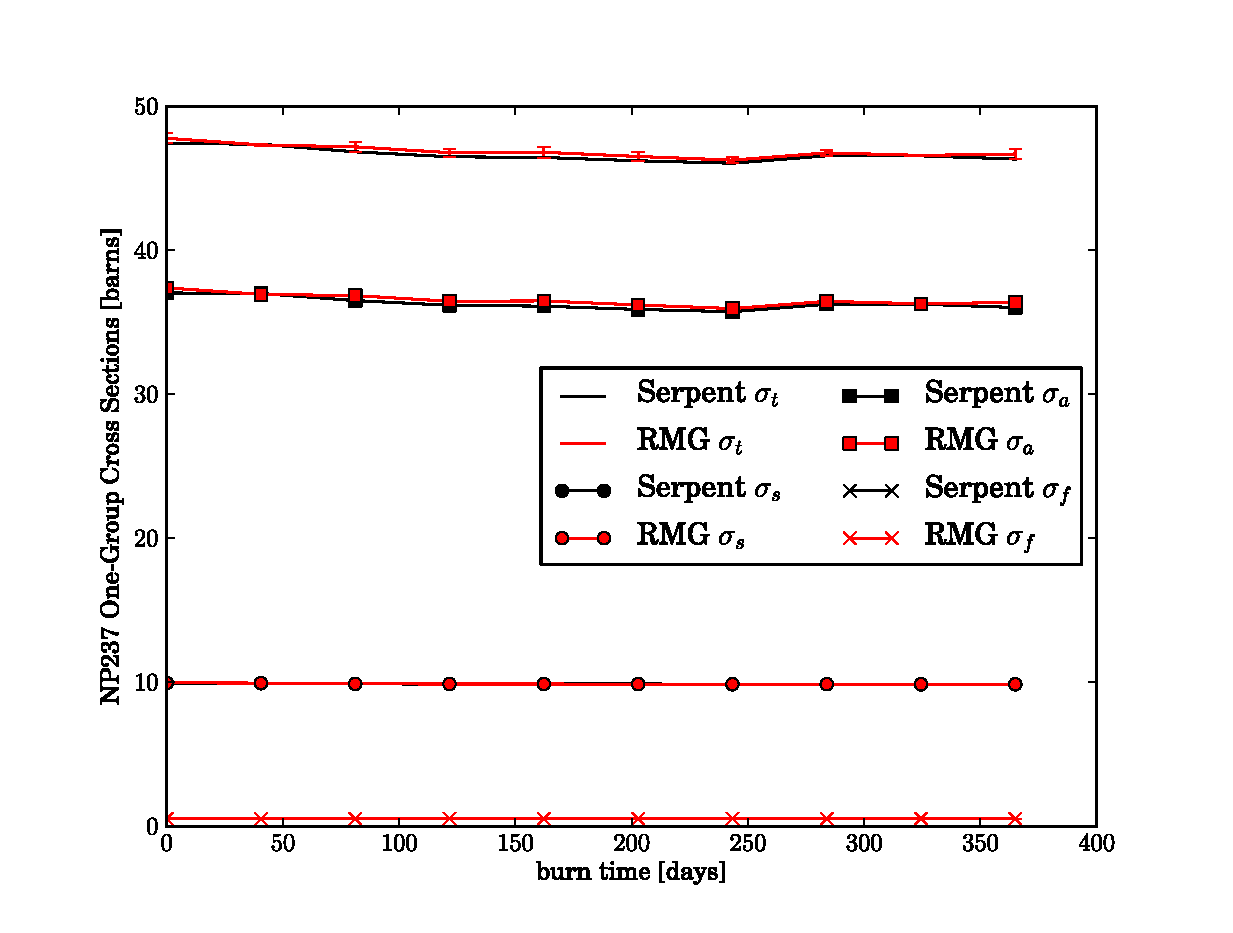
\includegraphics[scale=0.3]{multigroup_method/figs/benchmark/NP237_1g_xs.eps}
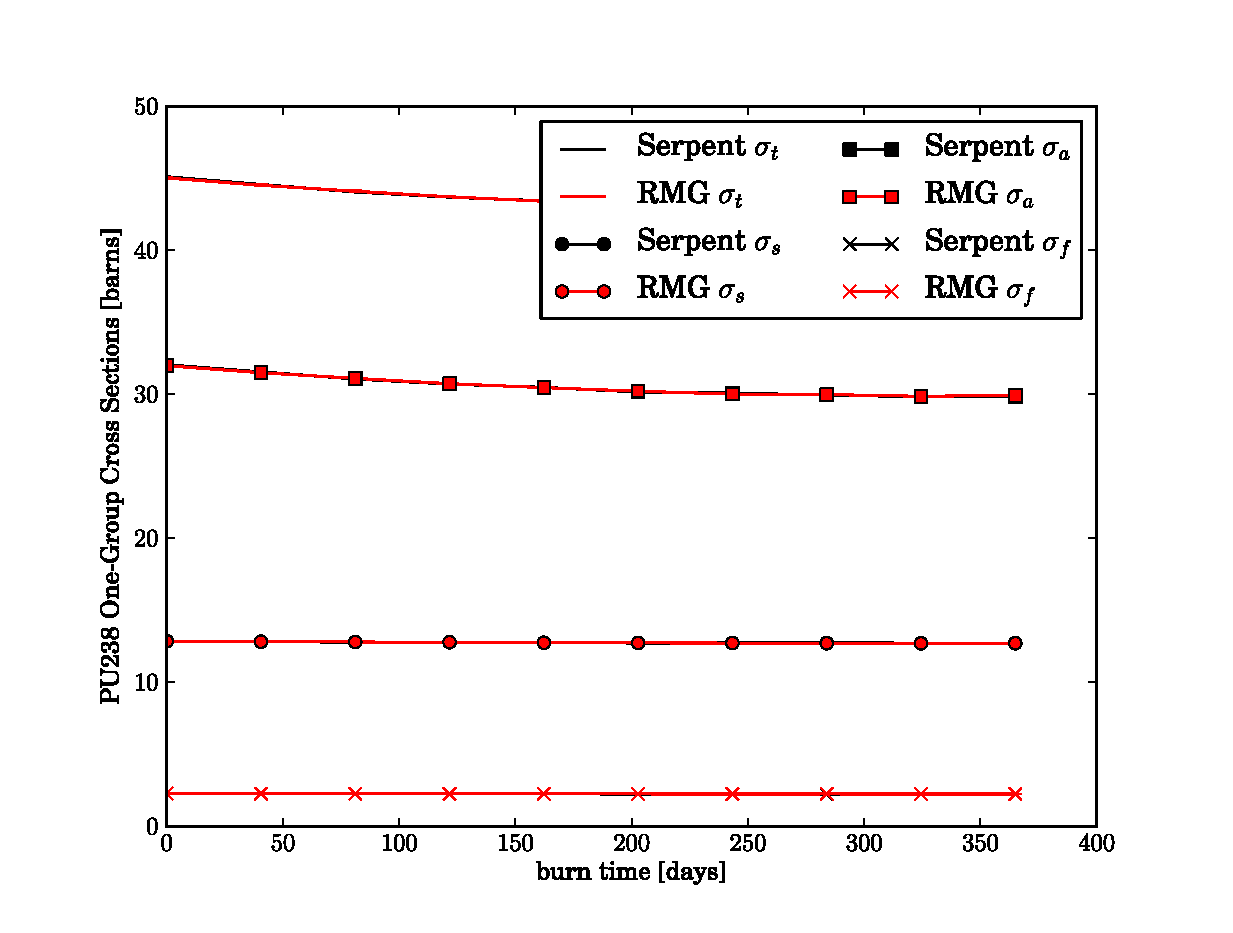
\includegraphics[scale=0.3]{multigroup_method/figs/benchmark/PU238_1g_xs.eps}
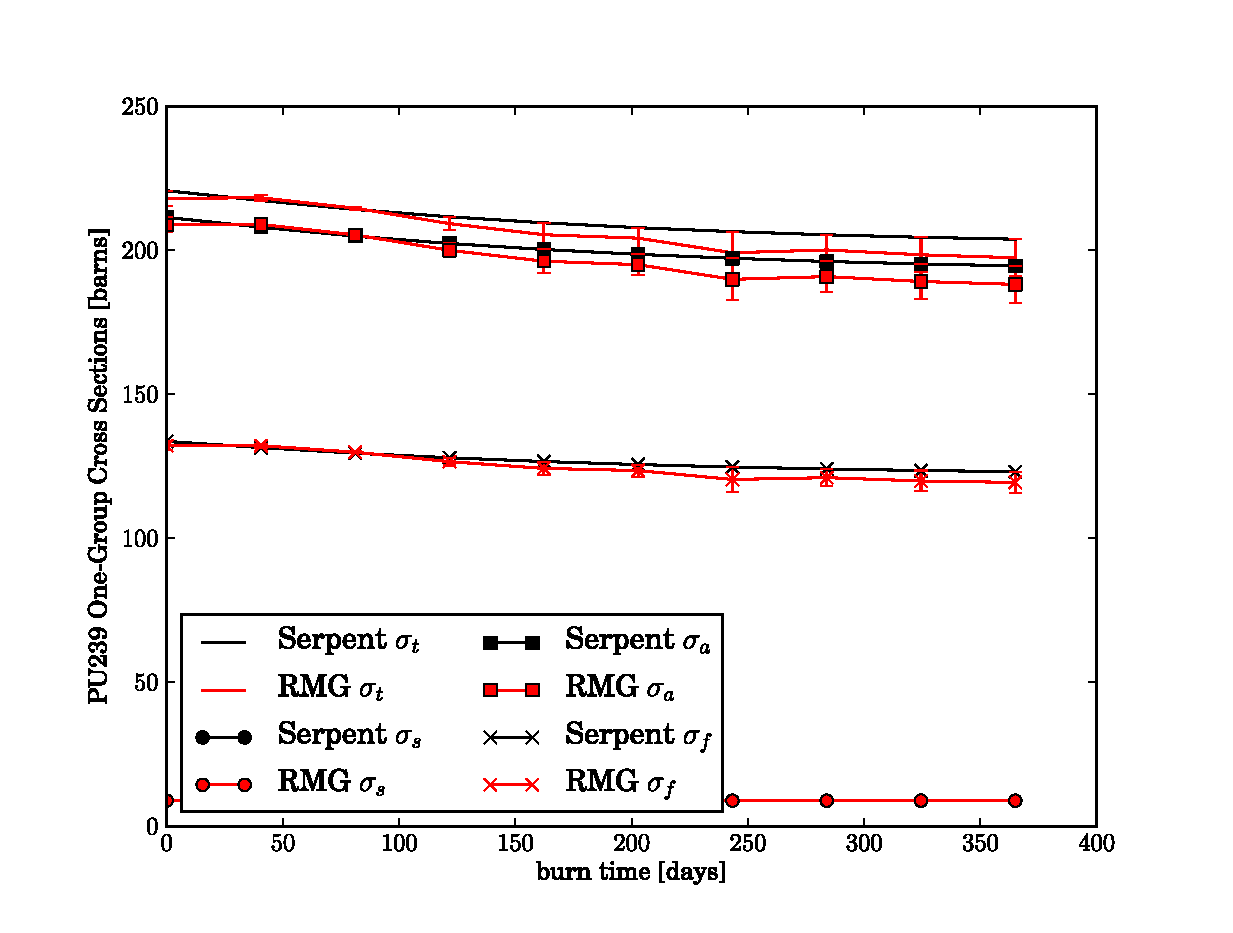
\includegraphics[scale=0.3]{multigroup_method/figs/benchmark/PU239_1g_xs.eps}
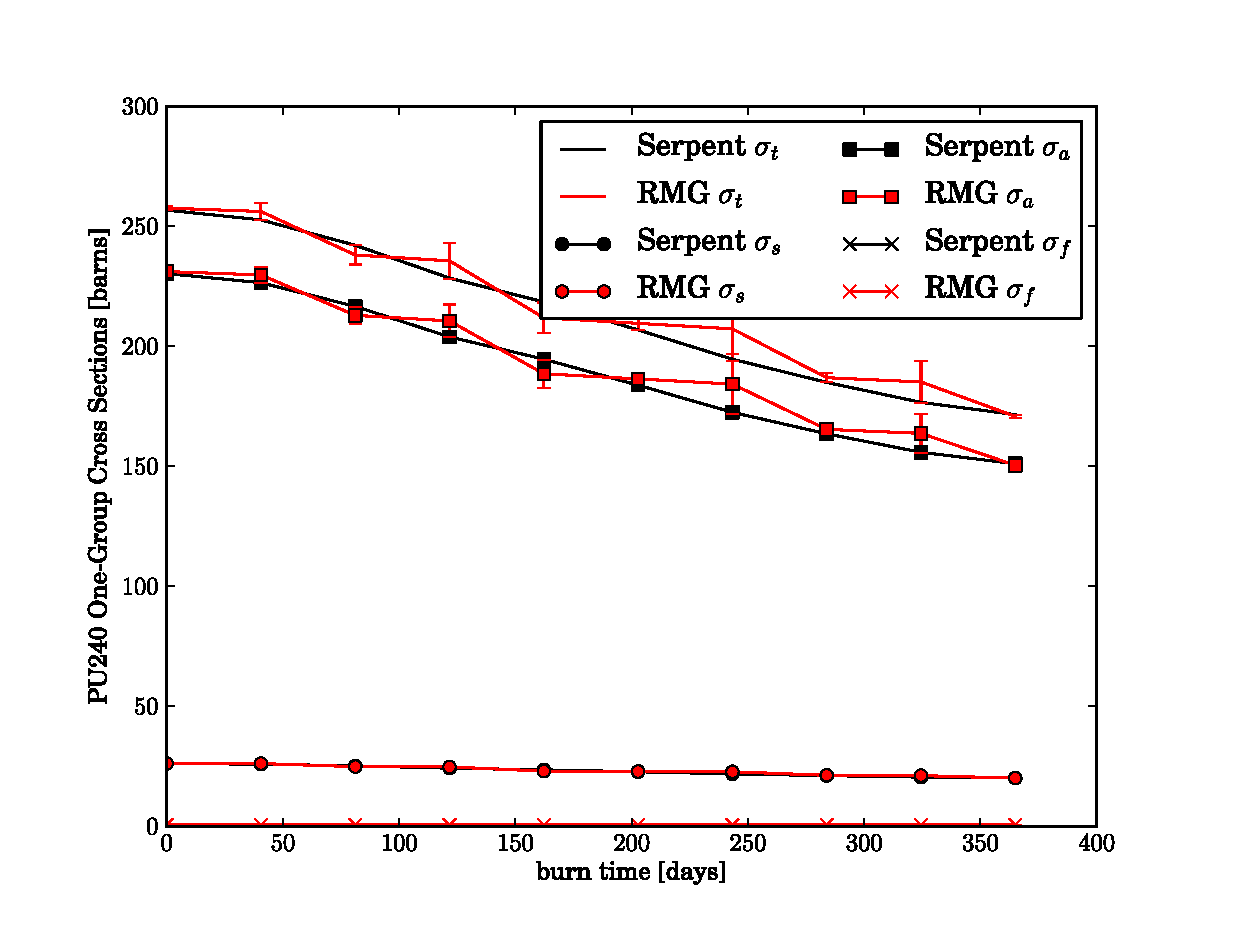
\includegraphics[scale=0.3]{multigroup_method/figs/benchmark/PU240_1g_xs.eps}
\end{center}
\end{figure}
\begin{figure}[htbp]
\caption{Actinide One-Group Cross-Section Benchmarks (Cont.)}
\label{act_xs_benchmark_cont}
\begin{center}
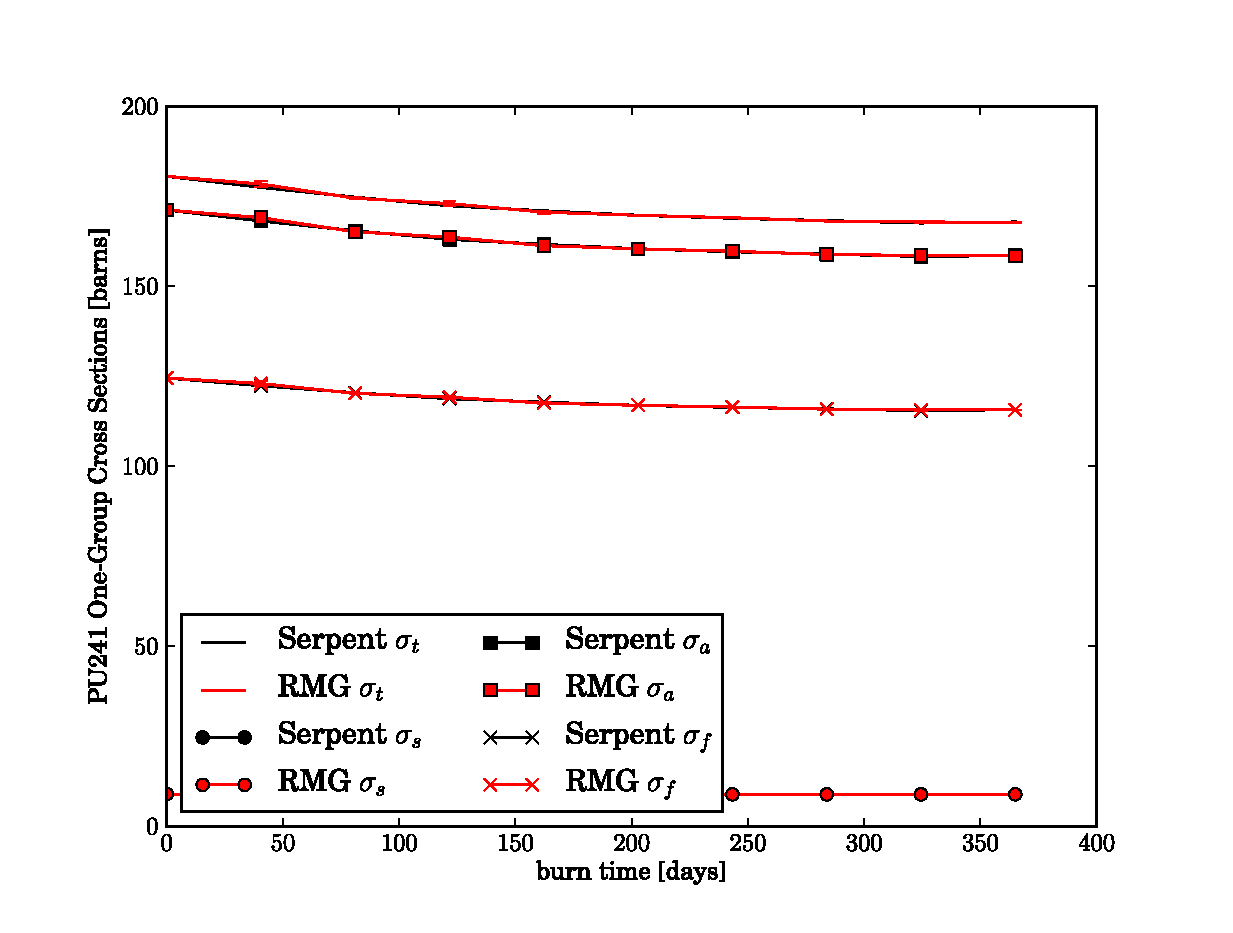
\includegraphics[scale=0.3]{multigroup_method/figs/benchmark/PU241_1g_xs.eps}
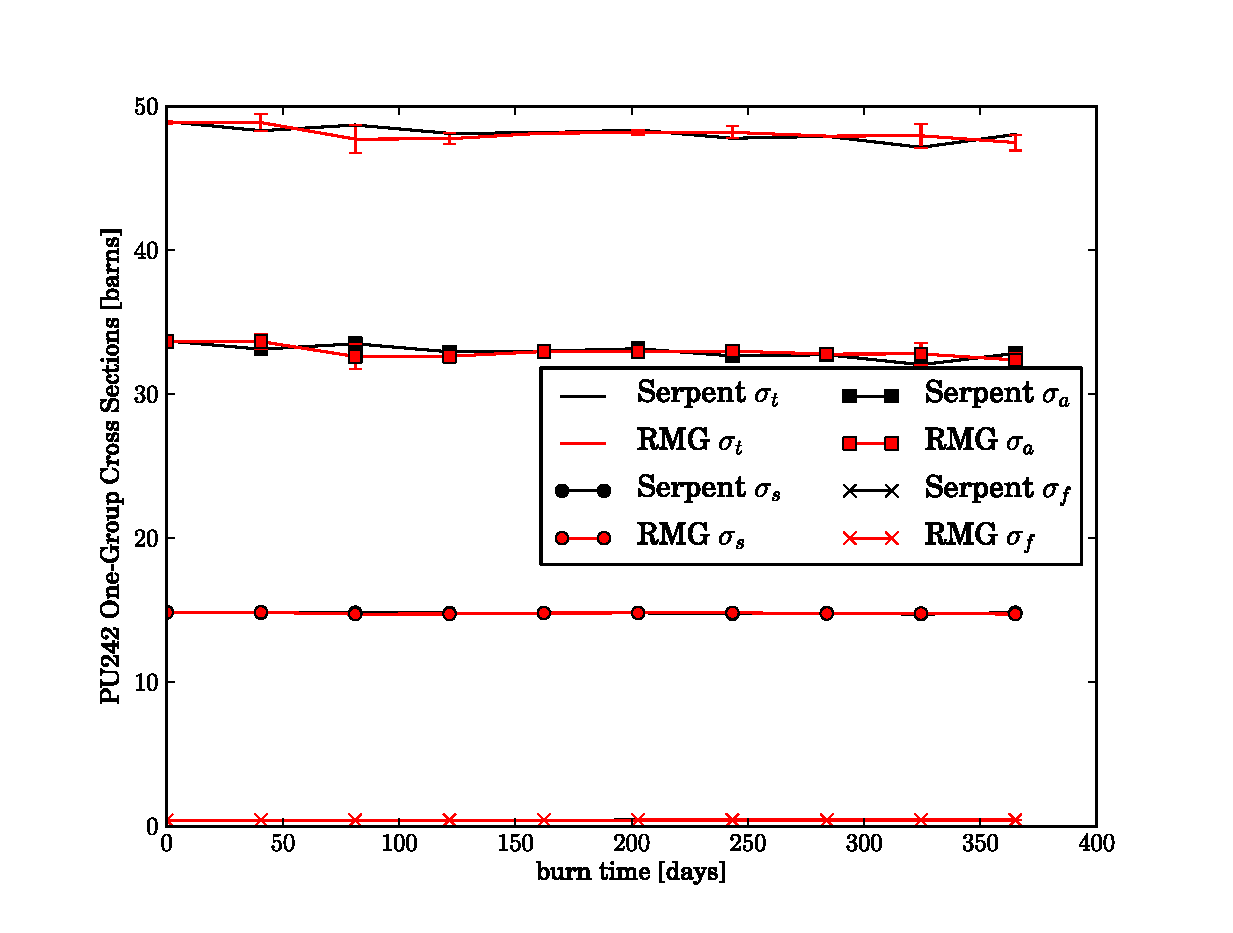
\includegraphics[scale=0.3]{multigroup_method/figs/benchmark/PU242_1g_xs.eps}
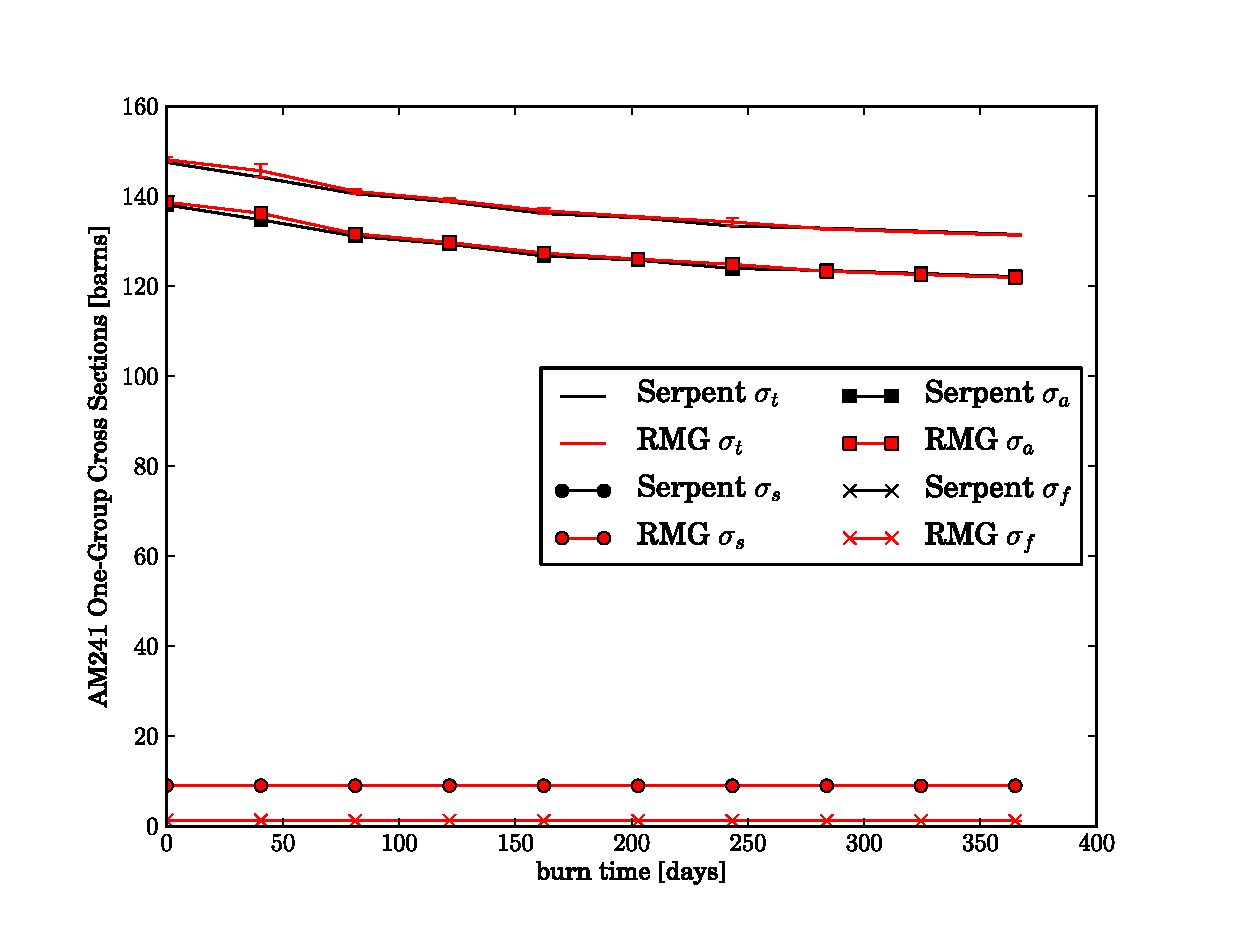
\includegraphics[scale=0.3]{multigroup_method/figs/benchmark/AM241_1g_xs.eps}
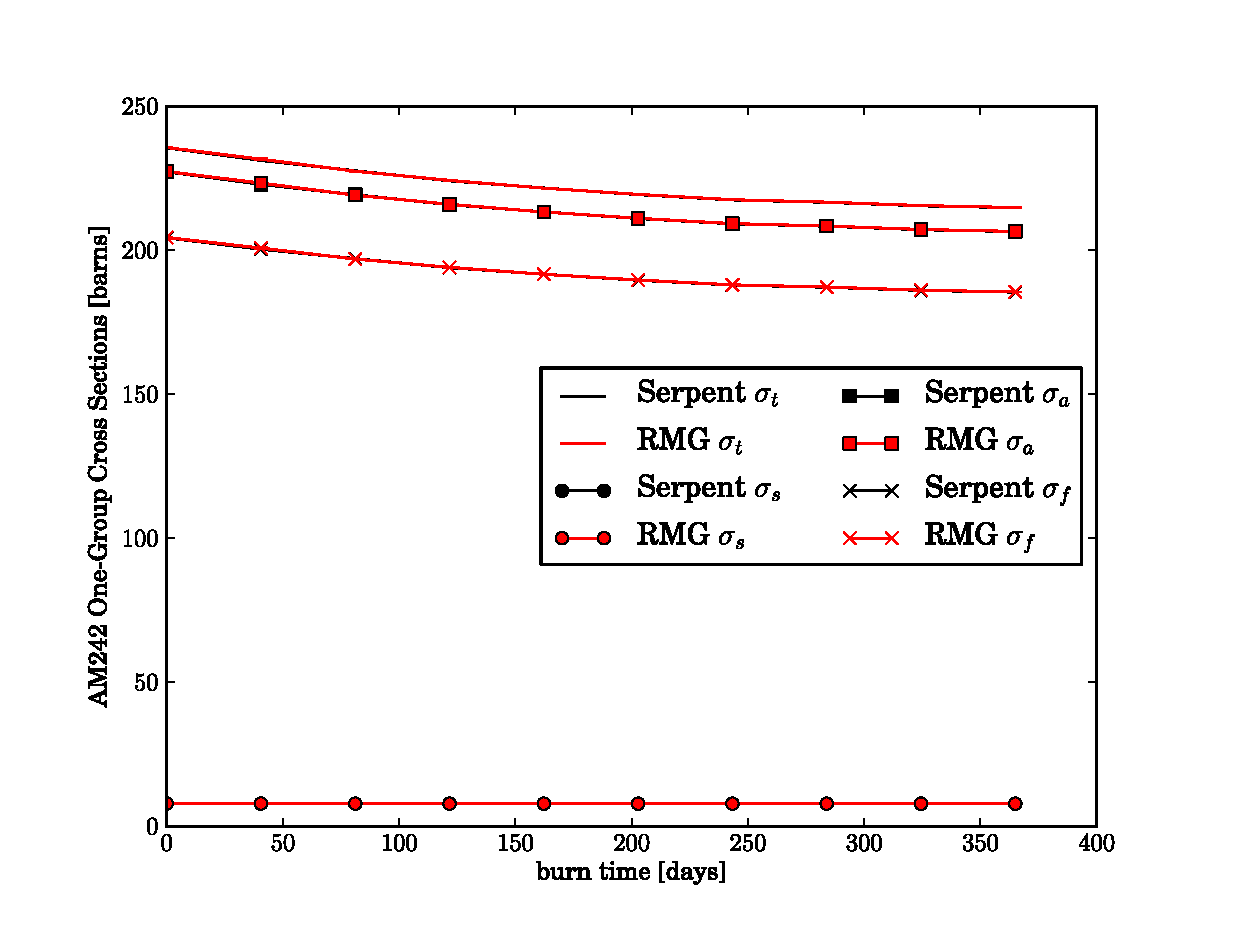
\includegraphics[scale=0.3]{multigroup_method/figs/benchmark/AM242_1g_xs.eps}
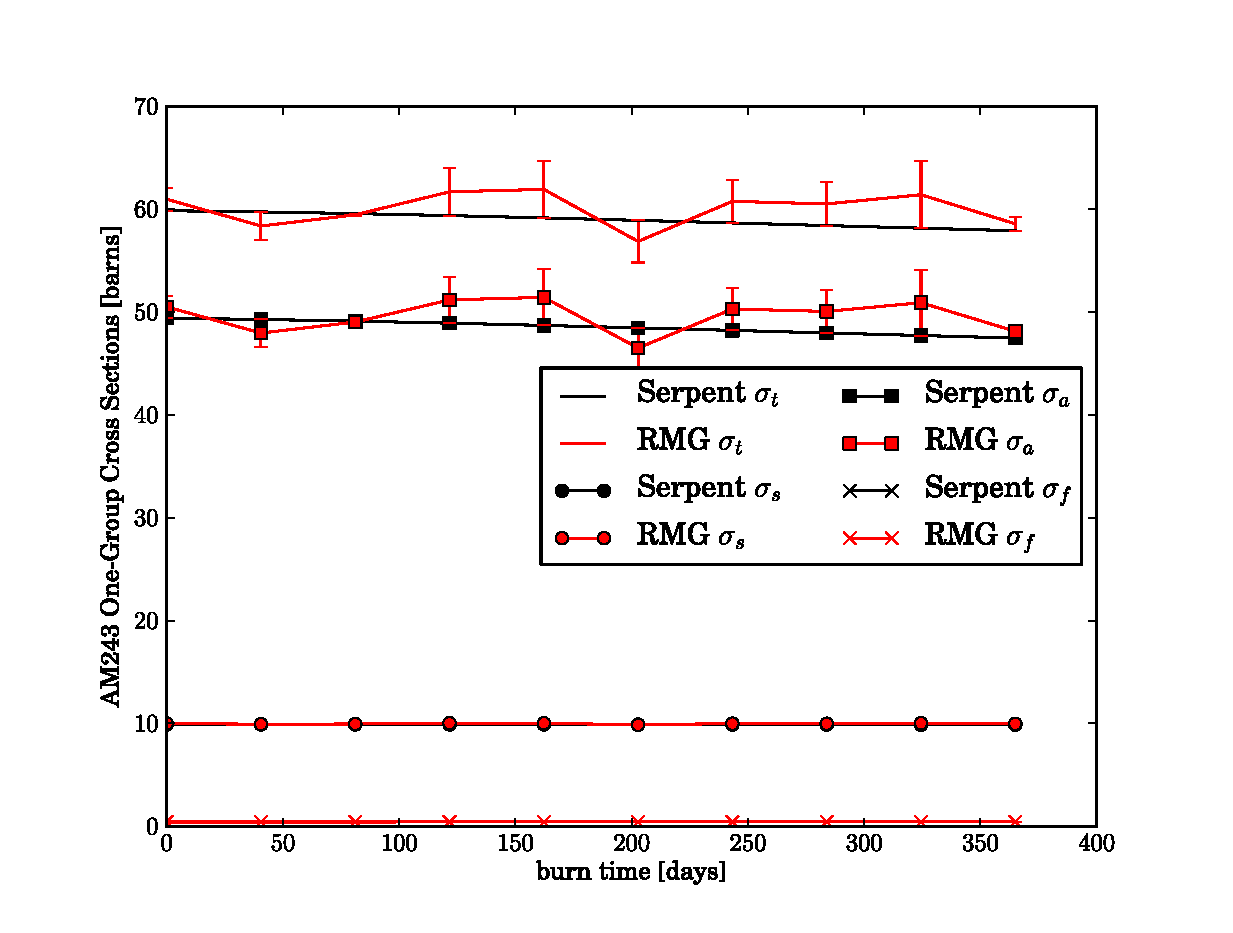
\includegraphics[scale=0.3]{multigroup_method/figs/benchmark/AM243_1g_xs.eps}
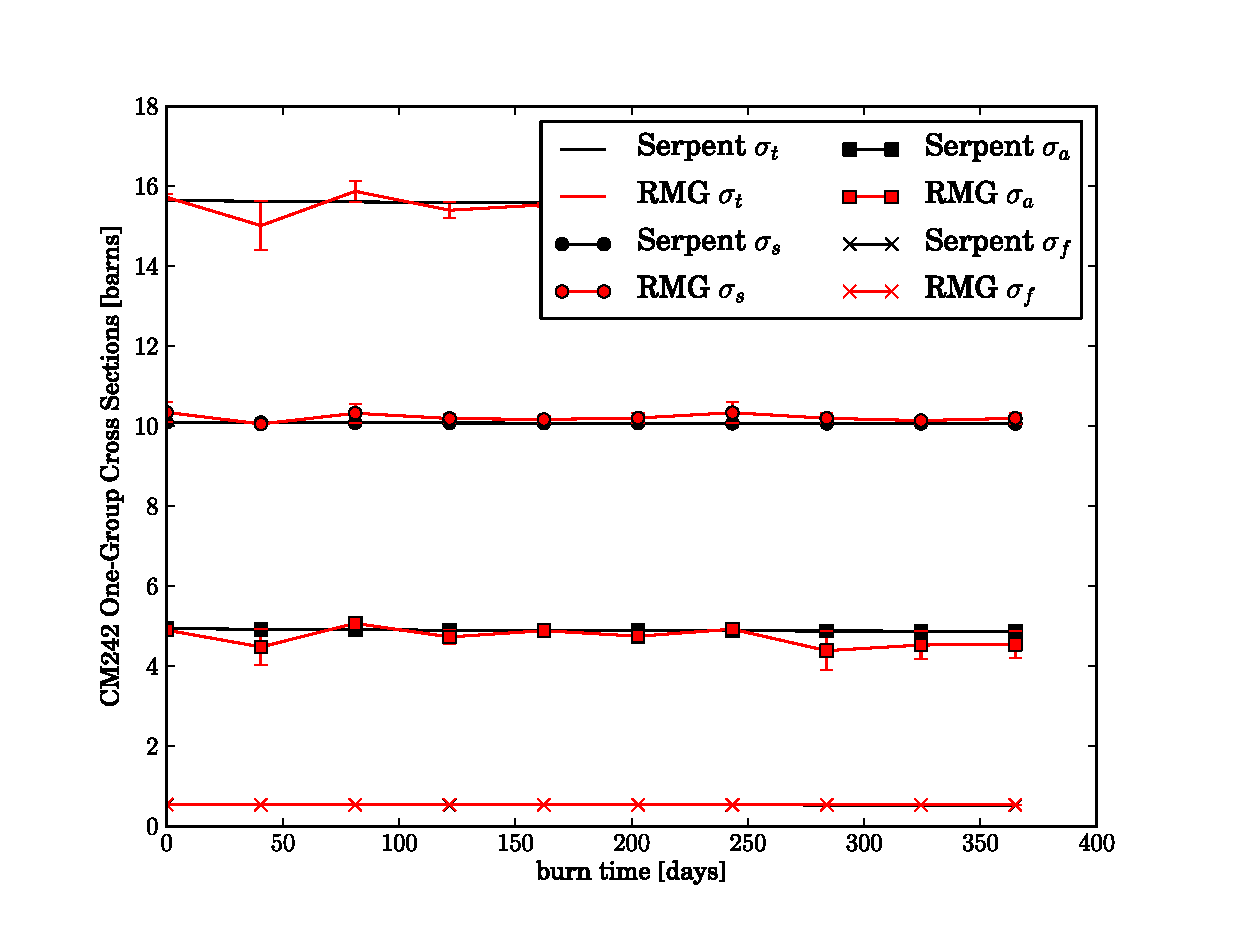
\includegraphics[scale=0.3]{multigroup_method/figs/benchmark/CM242_1g_xs.eps}
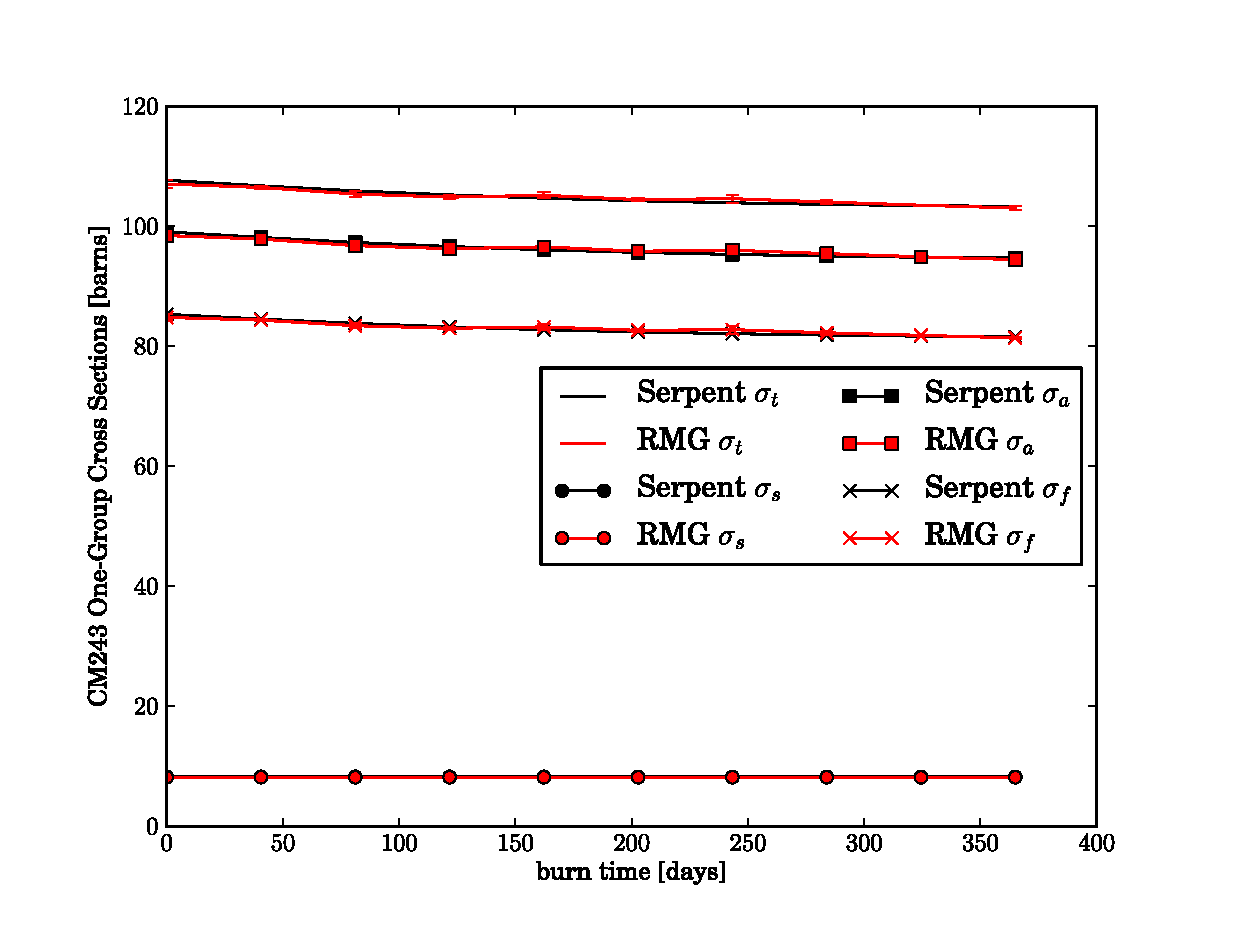
\includegraphics[scale=0.3]{multigroup_method/figs/benchmark/CM243_1g_xs.eps}
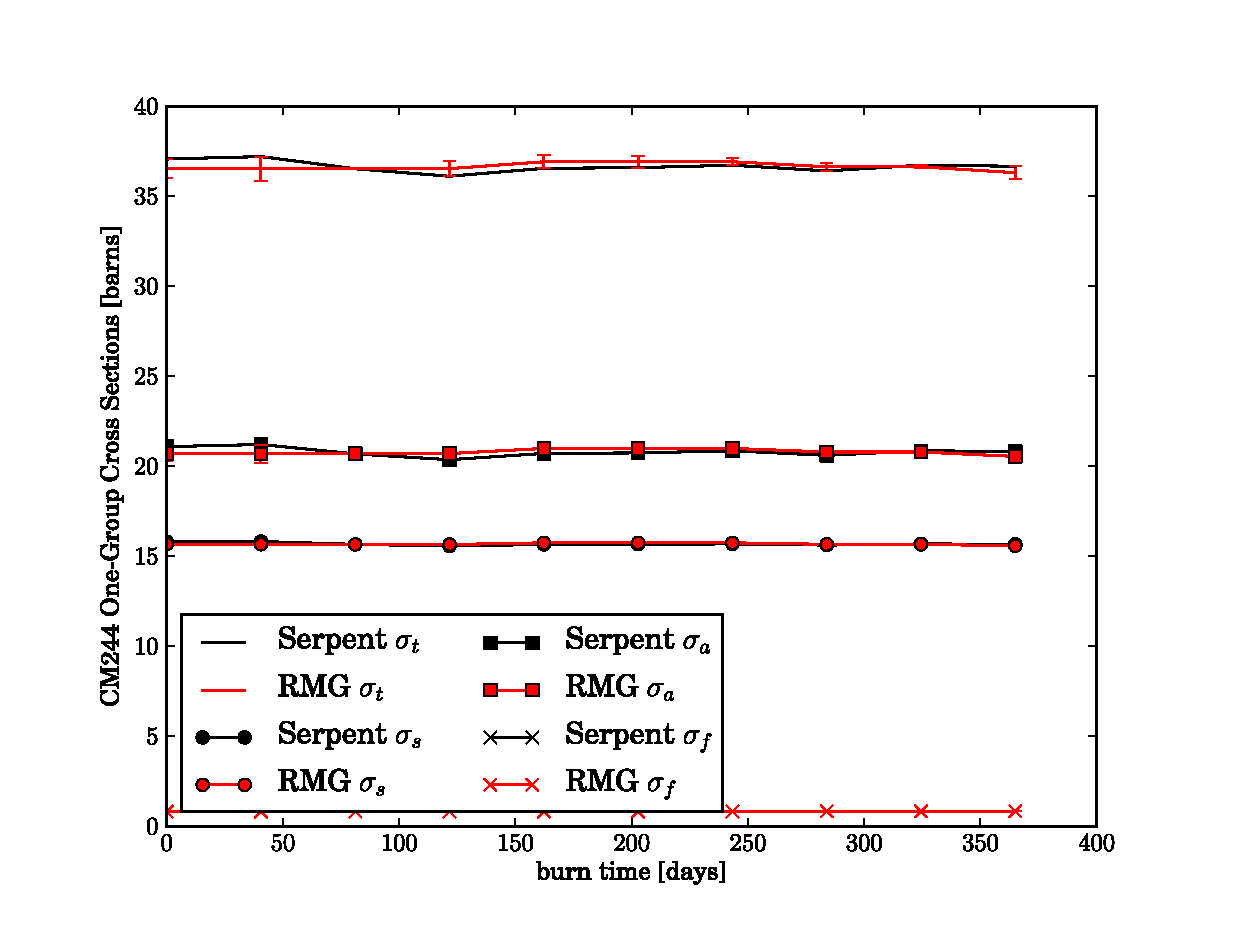
\includegraphics[scale=0.3]{multigroup_method/figs/benchmark/CM244_1g_xs.eps}
\end{center}
\end{figure}
\begin{figure}[htbp]
\caption{Actinide \& Fission Product One-Group Cross-Section Benchmarks}
\label{act_fp_xs_benchmark}
\begin{center}
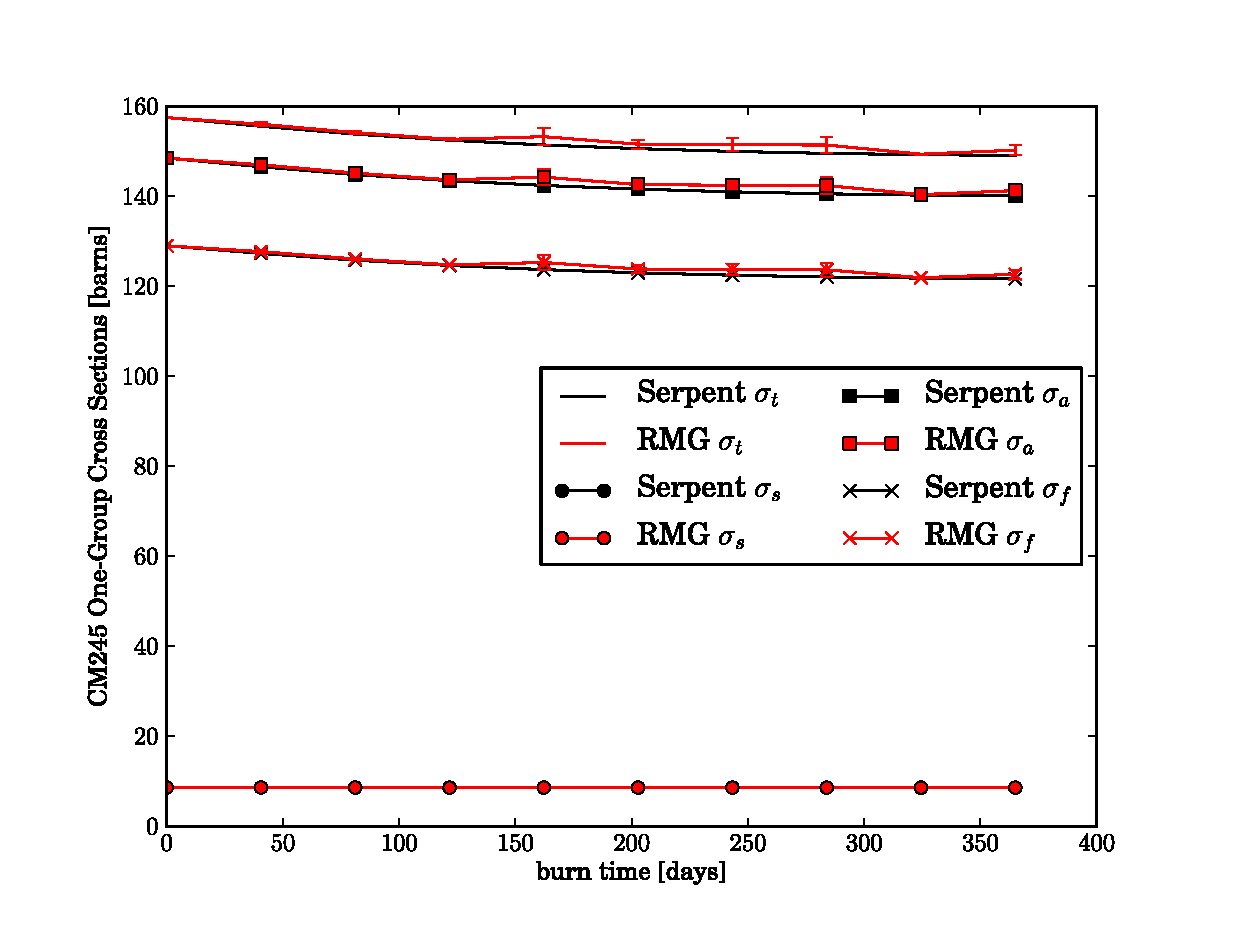
\includegraphics[scale=0.3]{multigroup_method/figs/benchmark/CM245_1g_xs.eps}
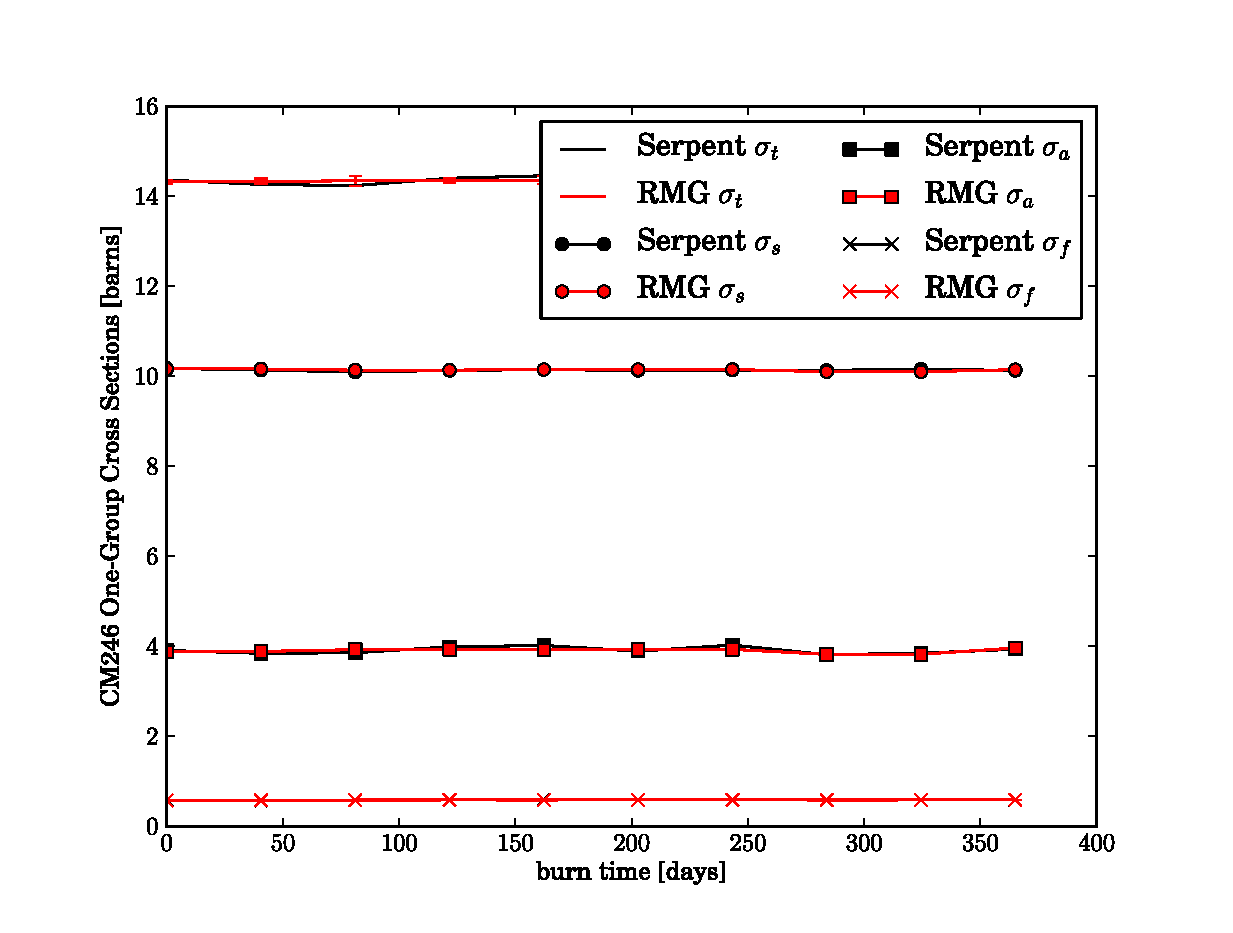
\includegraphics[scale=0.3]{multigroup_method/figs/benchmark/CM246_1g_xs.eps}
\includegraphics[scale=0.3]{multigroup_method/figs/benchmark/SE79_1g_xs.eps}
\includegraphics[scale=0.3]{multigroup_method/figs/benchmark/KR85_1g_xs.eps}
\includegraphics[scale=0.3]{multigroup_method/figs/benchmark/SR90_1g_xs.eps}
\includegraphics[scale=0.3]{multigroup_method/figs/benchmark/ZR93_1g_xs.eps}
\includegraphics[scale=0.3]{multigroup_method/figs/benchmark/TC99_1g_xs.eps}
\includegraphics[scale=0.3]{multigroup_method/figs/benchmark/I129_1g_xs.eps}
\end{center}
\end{figure}
\begin{figure}[htbp]
\caption{Fission Product One-Group Cross-Section Benchmarks}
\label{fp_xs_benchmark}
\begin{center}
\includegraphics[scale=0.3]{multigroup_method/figs/benchmark/PD107_1g_xs.eps}
\includegraphics[scale=0.3]{multigroup_method/figs/benchmark/CS134_1g_xs.eps}
\includegraphics[scale=0.3]{multigroup_method/figs/benchmark/CS137_1g_xs.eps}
\includegraphics[scale=0.3]{multigroup_method/figs/benchmark/SM151_1g_xs.eps}
\end{center}
\end{figure}

Lastly, since the one-group cross sections are feed to Origen to make a transmutation library, it is important 
to ensure that no library is reaction is far off from a benchmark value.  Tables 
\ref{rank_Actinide_sigma_s_table}-\ref{rank_Actinide_sigma_f_table} display the 
nuclides with the highest $\varepsilon$ (in decending order) at any time step for absorption and scattering
reactions for the fission products and for absorption, scattering and fission reactions for the actinides.
These tables have been filtered to remove species that have very short half lives within the reactor.
As Tables \ref{rank_Actinide_sigma_s_table}-\ref{rank_Actinide_sigma_f_table} display, even in the worst case 
the cross sections meet within acceptable levels or error.

\begin{table}[htbp]
\begin{center}
\caption{Maximum Actinide $\sigma_s$ Relative Error}
\label{rank_Actinide_sigma_s_table}
\begin{tabular}{|l|c|}
\hline
\textbf{Nuclide} & \textbf{$\varepsilon$} \\
\hline
\nuc{Pu}{240} & +0.0410 \\
\nuc{Cm}{244} & -0.0096 \\
\nuc{Pu}{242} & +0.0094 \\
\nuc{U}{236} & +0.0072 \\
\nuc{Cm}{246} & -0.0055 \\
\nuc{Pu}{238} & -0.0051 \\
\nuc{U}{234} & -0.0048 \\
\nuc{Cm}{242} & -0.0036 \\
\nuc{Pu}{239} & +0.0023 \\
\nuc{Pu}{241} & +0.0015 \\
\nuc{Am}{241} & +0.0015 \\
\nuc{Am}{243} & +0.0014 \\
\nuc{Np}{237} & +0.0014 \\
\nuc{Am}{242}\superscript{*} & -0.0014 \\
\nuc{U}{238} & +0.0012 \\
\nuc{Cm}{243} & -0.0008 \\
\nuc{Cm}{245} & -0.0005 \\
\nuc{U}{235} & -0.0005 \\
\hline
\end{tabular}
\end{center}
\end{table}

\begin{table}[htbp]
\begin{center}
\caption{Maximum Fission Product $\sigma_s$ Relative Error}
\label{rank_Fission_Product_sigma_s_table}
\begin{tabular}{|l|c|}
\hline
\textbf{Nuclide} & \textbf{$\varepsilon$} \\
\hline
\nuc{H}{1} & +0.4273 \\
\nuc{Eu}{155} & -0.2948 \\
\nuc{C}{14} & +0.2635 \\
\nuc{Ni}{63} & +0.2405 \\
\nuc{Cl}{36} & +0.2405 \\
\nuc{Nb}{91} & +0.2379 \\
\nuc{Nb}{93}\superscript{*} & +0.2377 \\
\nuc{Mo}{93} & +0.2377 \\
\nuc{Nb}{95}\superscript{*} & +0.2376 \\
\nuc{Tc}{98} & +0.2374 \\
\nuc{Ag}{108}\superscript{*} & +0.2367 \\
\nuc{Cd}{113}\superscript{*} & +0.2364 \\
\nuc{Sn}{117}\superscript{*} & +0.2362 \\
\nuc{Sn}{119}\superscript{*} & +0.2360 \\
\nuc{Sn}{121}\superscript{*} & +0.2359 \\
\nuc{Te}{125}\superscript{*} & +0.2357 \\
\nuc{Sm}{145} & +0.2347 \\
\nuc{Pm}{146} & +0.2347 \\
\nuc{Eu}{149} & +0.2345 \\
\nuc{Eu}{150} & +0.2345 \\
\hline
\end{tabular}
\end{center}
\end{table}

\begin{table}[htbp]
\begin{center}
\caption{Maximum Actinide $\sigma_a$ Relative Error}
\label{rank_Actinide_sigma_a_table}
\begin{tabular}{|l|c|}
\hline
\textbf{Nuclide} & \textbf{$\varepsilon$} \\
\hline
\nuc{U}{236} & -0.0513 \\
\nuc{Pu}{240} & +0.0493 \\
\nuc{Cm}{244} & -0.0312 \\
\nuc{Pu}{242} & -0.0263 \\
\nuc{Cm}{242} & +0.0231 \\
\nuc{Am}{242}\superscript{*} & +0.0231 \\
\nuc{Cm}{246} & +0.0203 \\
\nuc{Am}{243} & +0.0192 \\
\nuc{Pu}{239} & +0.0095 \\
\nuc{U}{234} & +0.0091 \\
\nuc{Am}{241} & +0.0078 \\
\nuc{Pu}{241} & +0.0054 \\
\nuc{Np}{237} & -0.0050 \\
\nuc{U}{238} & -0.0048 \\
\nuc{Pu}{238} & +0.0030 \\
\nuc{Cm}{245} & -0.0021 \\
\nuc{U}{235} & +0.0018 \\
\nuc{Cm}{243} & -0.0014 \\
\hline
\end{tabular}
\end{center}
\end{table}

\begin{table}[htbp]
\begin{center}
\caption{Maximum Fission Product $\sigma_a$ Relative Error}
\label{rank_Fission_Product_sigma_a_table}
\begin{tabular}{|l|c|}
\hline
\textbf{Nuclide} & \textbf{$\varepsilon$} \\
\hline
\nuc{Sn}{125} & +0.3476 \\
\nuc{Ba}{140} & +0.1934 \\
\nuc{Ba}{133} & -0.1820 \\
\nuc{Sm}{148} & +0.1529 \\
\nuc{Pm}{147} & -0.0992 \\
\nuc{Sb}{126} & +0.0965 \\
\nuc{Nb}{94} & -0.0716 \\
\nuc{Zr}{93} & -0.0622 \\
\nuc{Ni}{59} & +0.0374 \\
\nuc{Pd}{107} & +0.0315 \\
\nuc{Tc}{99} & -0.0312 \\
\nuc{Cs}{135} & -0.0311 \\
\nuc{Eu}{155} & +0.0235 \\
\nuc{Eu}{154} & -0.0169 \\
\nuc{Eu}{152} & -0.0151 \\
\nuc{Kr}{85} & -0.0135 \\
\nuc{Cd}{113}\superscript{*} & -0.0117 \\
\nuc{Eu}{149} & +0.0114 \\
\nuc{Sn}{126} & -0.0109 \\
\nuc{Eu}{150} & +0.0103 \\
\hline
\end{tabular}
\end{center}
\end{table}

\begin{table}[htbp]
\begin{center}
\caption{Maximum Actinide $\sigma_f$ Relative Error}
\label{rank_Actinide_sigma_f_table}
\begin{tabular}{|l|c|}
\hline
\textbf{Nuclide} & \textbf{$\varepsilon$} \\
\hline
\nuc{Cm}{247} & -0.1143 \\
\nuc{U}{236} & +0.0874 \\
\nuc{Cf}{252} & +0.0784 \\
\nuc{U}{232} & -0.0716 \\
\nuc{Cm}{248} & -0.0586 \\
\nuc{Th}{229} & -0.0525 \\
\nuc{Pu}{239} & +0.0511 \\
\nuc{Cf}{249} & -0.0441 \\
\nuc{Pu}{236} & +0.0420 \\
\nuc{Am}{241} & +0.0302 \\
\nuc{Th}{232} & -0.0298 \\
\nuc{Pu}{241} & +0.0295 \\
\nuc{Bk}{249} & +0.0260 \\
\nuc{Am}{242}\superscript{*} & -0.0239 \\
\nuc{Ac}{227} & -0.0219 \\
\nuc{Cf}{251} & -0.0218 \\
\nuc{Pu}{240} & +0.0206 \\
\nuc{U}{237} & +0.0150 \\
\nuc{U}{235} & +0.0108 \\
\nuc{Cm}{250} & +0.0103 \\
\hline
\end{tabular}
\end{center}
\end{table}



\section{Conclusion \& Future Work}
\index{Conclusion \& Future Work@\emph{Conclusion \& Future Work}}
The multigroup reactor model presented in this study provides a method for dynamically
computing group constants for any reactor state.  While the inital cross section library
generation stage may be computationally expensive (days), the resulting RMG calculations take
only a fraction of the time to execute (seconds).  This dramatic difference in time scales
makes the RMG well-suited to nuclear fuel cycle simulations.

Still, the RMG is subject to certain, natural constraints.  First, in moving from one- to $G$-groups,
the RMG will necessarily always take more computational resources to execute than the one-group
reactor model previously presented.  However, the benefit of using additional groups is that the flux
spectrum is allowed to change over the course of the fuel burn.  For fast reactors or standard light 
water reactor, changes in the spectrum are minimal so the error induced by the R1G from a static spectrum
is negligible.  On the other hand, the RMG enables appropriate modeling of forms such as inert matrix 
fuel for which R1G models would fundementally break.

Another constraint with the RMG as formulated is that a multidimensional linear interpolation is 
used when calculating $\sigma_{r_x,itg}$ from the reactor library $\sigma_{r_x,ipg}$.  Therefore, 
in order to capture non-linear effects in the cross sections, a refinement to the time grid may 
be required if the number of steps is too coarse in the area of interest.  This problem may be solved
in other ways as well.  Using a higher order polynomial fit or a spline interpolation would 
remove the use of a simple linear interpolation and may be more acurate.

Moreover, the perturbation table as formulated is static.  Simple cahnges to the table
require a complete re-computation of the outer product of all parameters.  While not computationally
intensive on its own, the perturbation table determines the state of the reactor and thus the 
value of all of the group constants in the reactor library.  In effect, it is the keystone of the RMG, 
as invalidating it invalidates all other parts of the reactor library.  

A more dynamic perturbation table, and thus more dynamic reactor library, would allow for the RMG to 
handle an increased number of reactor cases without causing a reset of all cases previously computed.
One method of implementation would be to allow the parameters in the pertubation table to be stochcatically
generated.  Each parameter $a_p$ would be given a range on which it would be randomly sampled to form a 
perturbation vector.  The exception to this is that burnup times would remain static and sequential, as
in the current formulation.  Such an implementation would enable the easy extention of the perturbation 
table (\emph{i.e.} adding rows).  Where this ability becomes particularly important is in the case 
where there are a large number of parameters, such as the strategy where the initial concentration of 
every actinide is varied.  Here, the option space is much more efficiently covered by a stochcastic 
perturbation table than an outer product one.

Lastly, refinements and optimizations to the existing model may be made.  For example, the current 
transmutation calculation is backed by Origen.  More sophisticated methods which minimize global error 
could be implemented into the RMG.  However, even the matrix exponential method used here is 
sufficient for most calculations.

In conclusion, the RMG satisfies the requirements of correctly handling changes in the neutron flux 
spectrum while mainiting comperable (though somewhat slower) runtimes to the one-group reactor model.
Future work will include the refinement mentioned above and the inclusion in a fuel cycle modeling 
framework.
